\documentclass[a4paper]{report}
\usepackage{amsmath,amssymb}
\usepackage{graphicx}
\usepackage{fancyhdr}

% این فایل شامل تنظیماتی است که قبل از لود شدن پکیج زی‌پرشین باید انجام شوند.
% دلیل آن است که نیاز به لود شدن یک پکیج (geometry) دارد، در حالی که bidi (که توسط زی‌پرشین
% لود می‌شود) حتما باید آخرین پکیج باشد. در نتیجه هر پکیج دیگری نیز که بخواهد لود شود، باید در این قسمت باشد.
% نسخه 1.0.7
% تاریخ: ۲۲ مهر ۱۳۹۳
% تغییرات: ۱) برای کارکردن با texlive2014 و زی‌پرشین جدید:
%               - فونتها با IRLotus جایگزین شدند => فقط با texlive2013 و texlive2014 کار می‌کند (با 2012
%                  کار نمی‌کند، چون کشیده و کاراکتر نیمفاصله را در خروجی بین دو عدد "" می‌گذارد!).
%               - بجای داشتن یک فایل MBZ_ThesisSettings.sty، دو فایل MBZ_ThesisSettings1.tex و
%                  MBZ_ThesisSettings1.tex داریم، که اولی شامل تنظیماتی است که قبل از لود کردن زی‌پرشین
%                  باید انجام شوند و دومی تنظیماتی که بعد از آن باید انجام شوند.

%%%%%%%%%%%%%%%%%%%%%%%%%%%%%%%%%%%%%%%%%%
% Start of Page Setup:
% تعریف متغیرها:
\newlength{\MyLeftMargin}
\newlength{\MyRightMargin}
\newlength{\MyTopMargin}
\newlength{\MyBottomMargin}

% اعداد در استاندارد تزهای دانشگاه شریف:
\setlength{\MyLeftMargin}{2.5cm}
\setlength{\MyRightMargin}{3cm} % -> Sharif says 3cm. I prefer 2.5.
\setlength{\MyTopMargin}{3cm}
\setlength{\MyBottomMargin}{2.5cm} % -> Sharif says 2.5cm. I prefer 2.7.

\usepackage[top=\MyTopMargin, bottom=\MyBottomMargin, left=\MyLeftMargin, right=\MyRightMargin]{geometry}
%\setlength{\columnwidth}{82mm}
%\setlength{\columnsep}{6mm}
% End of Page Setup
%%%%%%%%%%%%%%%%%%%%%%%%%%%%%%%%%%%%%%%%%% % All settings before xepersian (especially loading any other pachages,
                            % because xepersian should be the last loaded package.
							% written by Massoud Babaie-Zadeh
\usepackage[Kashida]{xepersian}
% این فایل شامل تنظیمات نوشته‌شده توسط اینجانب (مسعود بابایی‌زاده یا  MBZ) برای نوشتن تز یا گزارش است، چون خروجی پیش‌فرض xepersian اصلا تز زیبایی تولید نمی‌کند. همچنین دقت شود که از فونت MBZ Lotus و نیز پکیج digitfont (برای تغییر فونت ارقام به MBZ Lotus) که هر دو توسط اینجانب نوشته شدند به همراه این تنظیمات استفاده شود تا در نهایت خروجی زیبایی برای تز بدست آید.
% تنظیمات انجام شده در این فایل شامل موارد زیر هستند:
% اول: زیاد کردن فاصله خطوط در متن فارسی، کمتر زیاد کردن در ریاضی و متن انگلیسی: چون در XePersian زیادی خطوط توی هم هستند و زیبا نیست. این کار کار راحتی نبود و خیلی چیزها دست خوردند.
% دوم: فهرست مطالب در xepersian به نظرم اصلا زیبا نیست، چون در واقع چیز خاصی برای فارسی ندارد و از همان report استفاده می‌کند که برای زیبایی در انگلیسی طراحی شده نه فارسی. در نتیجه تغییرات متعددی در آن دادم تا فهرست مطالب به صورت زیباتری نوشته شود.
% سوم: تنظیم صفحات (page setup) ، یعنی حواشی بالا،‌ پایین، چپ و راست (پیش‌فرض طبق اعداد تزهای دانشگاه شریف).
% چهارم: تغییر فرمت header ، طوری که یک خط در آن کشیده شود و تیتر فصل و شماره صفحه بالای خط نوشته شود (fancy header).
% پنجم: نحوه تیتر گذاری شروع هر فصل تغییر داده شد: بالای آن با خط توخالی بنویسد (مثلا) «فصل ۱» و بعد زیر آن تیتر فصل را بنویسد و همه هم در وسط باشد. به نظرم از پیش‌فرض  report (که در واقع برای انگلیسی است) زیباتر است، لااقل برای تز.
% ششم: تغییر نحوه شماره‌گذاری فصلها و فرمولها و غیره، طوری که مثلا شماره فرمول به صورت (۱-۵) نوشته شود نه (۱.۵).
% هفتم: تغییر اینکه بجای «لیست اشکال» و «لیست جداول» بنویسد «فهرست اشکال» و «فهرست جداول».
% هشتم: تعریف دو محیط note (توجه) و experiment (آزمایش).
% نهم: تعریف محیطهایی مثل قضیه، تعریف و غیره (که نهایتا کامنت شده‌اند و غیرفعال هستند و کاربر اگر بخواهد می‌تواند آنها را فعال کند).
%
% نویسنده: مسعود بابایی‌زاده

% نسخه 1.0.9
% تاریخ: ۵ اسفند ۱۴۰۰
% تغییرات:
%   زی‌پرشینی که در دی وی دی texlive2021 بود (زیرپرشین نسخه 23.1) باگهای متعددی پیدا کرده است که تغییراتی که در این نسخه فایل حاضر داده شده است، همگی برای این است که فایل بتواند با این نسخه زی‌پرشین کار کند. اگر در نسخه‌های بعدی زی‌پرشین این مشکلات رفع شده باشد، بهتر است به نسخه قبلی (نسخه 1.0.8) برگشت. مشکلات زی‌پرشین جدید و تغییرات فایل حاضر برای رفع آنها عبارتند از:
%
%      ۱) این زی‌پرشین با فونت XB Titre Shadow که من برای نوشتن کلمه فصل (مثلا نوشتن کلمه «فصل ۱» بالای عنوان فصل اول) استفاده کرده بودم درست کار نمی‌کرد و آن را به صورت منفصل می‌نوشت («ف‌ص‌ل ۱»). پس این فونت را با IRSina جایگزین کردم (البته فونتهای خیلی زیادی امتحان کردم، بخصوص توخالی. ولی هیچدام جالب نبودند. شاید Mj_Nazila 3D Shadow بد نبود، ولی اعدادش بجای فارسی، عربی بودند). به هر حال به نظرم همان XB Titre Shadow خیلی بهتر است و چون ظاهرا این مشکل از خود زی‌پرشین است و نه فونت، در نسخه‌های آینده زی‌پرشین دقت شود که اگر این مشکل درست شده بود، مجددا به فونت XB Titre Shadow برگردیم.
%
%      ۲) صدا زدن دستور \setmathdigitfont در زی‌پرشین جدید منجر به یک خطای کمپایل می‌شود! راه حل پیشنهاد شده در لینک زیر در فایل حاضر استفاده شد:
%    http://qa.parsilatex.com/35710/__xepersian_mathsdigitspec_primitive_font_char_if_exist
%
%      ۳) محیط جدید document که با دستور زیر تعریف کرده بودم، در زی‌پرشین جدید این خطای کمپایل را می‌داد که \begin{olddocument} یا \end{document} تمام شده است!
%    \renewenvironment{document}{\begin{olddocument}\setlength{\baselineskip}{1.53\baselineskip}}{\end{olddocument}}
% که به وضوح باگ زی‌پرشین جدید است. در نتیجه دستور بالا را جایگرین کردم با دستور زیر:
%    \renewenvironment{document}{\olddocument\setlength{\baselineskip}{1.53\baselineskip}}{\endolddocument}


%%%%%%%%%%%%%%%%%%%%%%%%%%%%%%%%%%%%%%%%%%
% نسخه 1.0.8
% تاریخ: ۵ اسفند ۱۴۰۰
% تغییرات:
% تغییرات:
%           ۱) فونتهای پیش‌فرض متن که قبلا IRLotus بودند با IRLotusICEE (که نسخه اصلاح‌شده‌ای از IRLotus است که خودم برای کنفرانس برق ایران سال ۲۰۱۵ درست کرده بودم)، تغییر داده شد (ابتدا MBZLotus را هم اضافه کرده بودم، ولی در محیط itemize کار نمی‌کند و کاراکتر بولت آیتم را ندارد. در نتیجه حذف شد).
%
%           ۲) دستور \setdigitfont با \setmathdigitfont جایگزین شد تا با زی‌پرشین جدید درست کار کند و در عنوان فصلها، مثلا در  عبارت «فصل ۱»، عدد ۱ هم با همان فونت کلمه «فصل» (یعنی توخالی) نوشته شود، نه توپر.
%		   
%		   ۳) شماره‌گذاری فرمولها و زیرفصلها و غیره درست شد تا در زی‌پرشین جدید درست کار کند (وگرنه مثلا شماره فرمول ۲ فصل ۱، بجای (۲-۱) نوشته می‌شد (۱-۲)).

%%%%%%%%%%%%%%%%%%%%%%%%%%%%%%%%%%%%%%%%%%

% نسخه 1.0.7
% تاریخ: ۲۲ مهر ۱۳۹۳
% تغییرات: ۱) برای کارکردن با texlive2014 و زی‌پرشین جدید:
%               - فونتها با IRLotus جایگزین شدند => فقط با texlive2013 و texlive2014 کار می‌کند (با 2012
%                  کار نمی‌کند، چون کشیده و کاراکتر نیمفاصله را در خروجی بین دو عدد "" می‌گذارد!).
%               - بجای داشتن یک فایل MBZ_ThesisSettings.sty، دو فایل MBZ_ThesisSettings1.tex و
%                  MBZ_ThesisSettings2.tex داریم، که اولی شامل تنظیماتی است که قبل از لود کردن زی‌پرشین
%                  باید انجام شوند و دومی تنظیماتی که بعد از آن باید انجام شوند.
%          ۲) تعریف فونتهایی که در فایل Jeld.tex بود به همان MBZ_ThesisSettings2.tex منتقل شدند. اکنون همه
%             فونتها در همین فایل تعریف می‌شوند.
%          ۳) شماره گذاری حرفی طوری تغییر یافت که بجای «آ-ب-ج-د...» داشته باشیم «الف-ب-ج-د...» (با استفاده
%             از دستورات دکتر امین‌طوسی در تمپلیت دانشگاه خودشان.


%%%%%%%%%%%%%%%%%%%%%%%%%%%%%%%%%%%%%%%%%%
% نسخه‌های قبلی:
%%%%%%
% نسخه 1.0.6
% تاریخ: ۲۵ بهمن ۱۳۸۸
% تغییرات: ۱) تعریف محیط‌های definition، theorem، و ...
%           ۲) نحوه شماره‌گذاری table را فراموش کرده بودم که مثل figure درست کنم، اصلاح شد.
% ------>   3) bbding و محیط experiment درست شوند.  <-------
%           ۴) \headheigh هم تنظیم شد (برابر ۱۳ پوینت). قبلا اصلا دست نزده بودم، ظاهر پیش‌فرض آن ۱۲ بوده و fancyhdr وارنینگ می‌داد.
%%%%%%
% نسخه 1.0.5
% تاریخ: ۲۰ بهمن ۱۳۸۸
% تغییرات: در فهرست عنوان فصلها را بجای اینکه \Large بنویسم، کمی کوچکتر یعنی \large نوشتم (و عنوان \part ها کماکان \Large است).
%%%%%%
% نسخه 1.0.4
% تاریخ: ۱۸ بهمن ۱۳۸۸
% تغییرات: فونت تیتر فصلها را عوض کردم و طوری نوشتم که دو فونت متفاوت بگیرد، یکی برای شماره فصل (مثلا «فصل اول») و دیگری برای عنوان فصل (مثلا «مقدمه»). همچنین اولی را} XB Titre Shadow و دومی را Titre گذاشتم.

%%%%%%
% نسخه 1.0.3
% تاریخ: ۱۶ بهمن ۱۳۸۸
% تغییرات: نحوه نوشتن part را هم در فهرست عوض کردم، تا در فارسی زیبا شود. همچنین در فهرست اندازه تیتر فصلها را نیز از \Large به \large کاهش دادم، و اندازه تیتر part را به \Large نوشتم.
%%%%%%
% نسخه 1.0.2
% تاریخ: ۱۵ بهمن ۱۳۸۸
% تغییرات: فاصله فرمولها از متن بیشتر شد (به نظرم این فاصله را زیادی کم کرده بودم). کامنتهای بالا هم ترتیبشان تغییر کرد و تا حدودی به ترتیب اولویت شدند.

%%%%%%
% نسخه: ۱.۰.۱
% تاریخ: ۲۵ دیماه ۱۳۸۸ برابر با ۱۵ ژانوبه ۲۰۱۰
% تغییرات: تغییر داده شده نسبت به نسخه 1.0.0 فقط زیادکردن \parindent است. مقدار پیش‌فرض قبلی، برای متون انگلیسی است و در متون فارسی زیادی کوچک است.

%%%%%%%%%%%%%%%%%%%%%%%%%%%%%%%%%%%%%%%%%%
% Font settings

%\defpersianfont\chaptertitlenumberfont[Scale=1.31]{B Koodak Outline}
%\defpersianfont\chaptertitlenumberfont[Scale=1]{XB Titre Shadow}
\defpersianfont\chaptertitlenumberfont[Scale=1]{IRSina.ttf}
\defpersianfont\chaptertitlefont[Scale=1]{IRTitr.ttf}

% فونت اصلی متن فونت «یاس» است که توسط کاربران xepersian از اصلاح XB Yas به دست آمده است.
%\settextfont[Scale=1.1]{IRLotus}
%\setlatintextfont[Scale=1]{Times New Roman}
%\setonlydigitfont[Scale=1.1]{Yas} %This is not a xepersian command. It is a command provided by setdigitfont.sty, written by Massoud Babaie-Zadeh
%\setdigitfont[Scale=1.1]{IRLotus}

% استفاده از حالت خوابیده به چپ قلم «یاس» مشابه با حالت ایرانیک در فارسی‌تک
%\setiranicfont[Scale=1.1]{IRLotus-Italic}

% 12 point "IRLotus" is small. Use 13.1 point (which gives a size similar to FarsiTeX)
\settextfont[ BoldFont={IRLotusICEE_Bold.ttf}, BoldItalicFont={IRLotusICEE_BoldIranic.ttf}, ItalicFont={IRLotusICEE_Iranic.ttf},Scale=1.31]{IRLotusICEE.ttf}%{IRZar.ttf}
%\setdigitfont[Scale=1.31]{IRLotusICEE} % replaced by the next command since texlive2018:
% دستور بالا از نسخه‌ای به بعد زی‌پرشین (لااقل از texlive2018 به بعد) باعث میشود که همه عددها با فونت بالا جایگزین شود که مطلوب نیست. مثلا در عنوان فصل که نوشته شده «فصل ۱» هم کلمه «۱» با این فونت (و در نتیجه توپر) نوشته میشود در حالیکه «فصل» با فونت توخالی بوده. و برای اینکه فقط اعداد داخل فرمولها فارسی شوند، دستور بالا با دستور جدید \setmathdigitfont در زیر جایگزین شد:

% شروع دستوراتی برای رفع یک باگ در زی‌پرشین 23.1 که در دی وی دی texlive2021 است. منبع: http://qa.parsilatex.com/35710/__xepersian_mathsdigitspec_primitive_font_char_if_exist
\ExplSyntaxOn
\cs_set_eq:NN
\etex_iffontchar:D
\tex_iffontchar:D
\cs_undefine:N \c_one
\int_const:Nn \c_one { 1 }
\ExplSyntaxOff
% پایان دستورات رفع باگ بالا در زی‌پرشین 23.1
\setmathdigitfont[Scale=1.31]{IRLotusICEE.ttf}
%\setlatintextfont[Scale=1]{Times New Roman}
\setiranicfont[Scale=1.31]{IRLotusICEE_Iranic.ttf}				% ایرانیک، خوابیده به چپ

% Fonts on JELD (title page)
\defpersianfont\mainjeldfont[ BoldFont={IRLotusICEE_Bold.ttf}, BoldItalicFont={IRLotusICEE_BoldIranic.ttf}, ItalicFont={IRLotusICEE_Iranic.ttf},Scale=1.31]{IRLotusICEE.ttf}
\defpersianfont\fieldnamefont[Scale=1.2]{BKoodakO.ttf}
\defpersianfont\ITRCthanksfont[Scale=1]{BTraffic.ttf}


%%%%%%%%%%%%%%%%%%%%%%%%%%%%%%%%%%%%%%%%%%
% دستور بعدی برای زیادکردن فاصلهٔ بین خطوط نوشته شده بود:
%\renewcommand{\baselinestretch}{2.3}
%\setstretch{2.3}
%\linespread{2.3}

% در اینصورت مشکل آن است که نه تنها فاصله بین خطوط متون فارسی را زیاد کنیم، فاصله خطوط بین فرمولها (مثلا در ماتریسها) هم زیاد می‌شود (که عدد ۲.۳ بالا زیادی بزرگ است). بعد برای حل این مشکل ابتدا سعی کردم محیط equation را طوری تغییر دهیم که اول فاصله خطوط را کمتر کند، بعد equation قدیم را صدا بزند. من متناسب با فاصله خطوط فارسی برابر 2.3 برابر (عدد بالا) فاصله فرمولها برابر 1.5 به نظرم خوب آمد، پس اول همه این دستورات را امتحان کردم:
%\let\oldequation=\equation
%\let\endoldequation=\endequation
%\renewenvironment{equation}{\vspace{-1em}\begin{spacing}{1.5}\begin{oldequation}}{\end{oldequation}\end{spacing}\vspace{-1em}}

%\renewenvironment{equation}{\begingroup\setstretch{1}\begin{oldequation}}{\end{oldequation}\setstretch{2.3}\endgroup}

%\renewenvironment{equation}{\vskip -\parskip\vskip -\baselineskip\begin{spacing}{1.5}\begin{oldequation}}{\end{oldequation}\end{spacing}\vskip -\parskip\vskip -\baselineskip}

%\renewenvironment{equation}{\begin{spacing}{1.5}\begin{oldequation}}{\end{oldequation}\end{spacing}}

%\let\old\baselinestretch=\baselinestretch\renewcommand{\baselinestretch}{2.3}
%\renewenvironment{equation}{\begingroup\def\baselinestretch{1.5}\begin{oldequation}}{\end{oldequation}\def\baselinestretch{2.3}\endgroup}

 % اما هر کدام مشکلی داشت. بهتر از همه همان اولی بود که مشکل آن این بود که پاراگراف بعد از فرمولها همیشه indent می‌شود.

% در نهایت راه حل بهتری پیدا کردم. متوجه شدم که زیاد کردن \baselineskip بر خلاف \baselinestreatch روی محیط ریاضی تاثیری ندارد. اما \baselineskip را باید بعد از \begin{document} زیاد کرد. با توجه به اینکه singlespace برای فرمولهای ریاضی در متن فارسی ما زیادی کوچک است،‌ پس برای آنکه طبق اعداد بالا فاصله خطوط در فرمولهای 1.5 برابر و در متن فارسی 2.3 برابر باشد، لازم است که طبق دستور زیر \baselinestreatch برابر 1.5 قرار داده شود و سپس درون متن و بعد از  \begin{document} باید \baselineskip را 2.3/1.5=1.53 برابر نمود. یعنی:

\renewcommand{\baselinestretch}{1.5}
%\setlength{\baselineskip}{1.53\baselineskip}   ->  This is inside the text and right after \begin{document}
%برای آنکه کاربر مجبور نباشد دستور بالا را دستی بعد از begin document اضافه کند، دستورات زیر را می‌نویسیم:
\let\olddocument=\document
\let\endolddocument=\enddocument
%\renewenvironment{document}{\begin{olddocument}\setlength{\baselineskip}{1.53\baselineskip}}{\end{olddocument}}
\renewenvironment{document}{\olddocument\setlength{\baselineskip}{1.53\baselineskip}}{\endolddocument}
%در اینصورت متوجه شدم که فاصله فرمولها با متن کمی زیاد می‌شود که آن را نیز با دستورات زیر می‌توان حل کرد (عدد 0.5em در نسخه 1.0.2 گذاشته شد، قبلا بالا را -0.6em و پایین را 0.7em گذاشته بودم که به نظرم فرمولها زیادی به متن نزدیک می‌شد):
\let\oldequation=\equation
\let\endoldequation=\endequation
\renewenvironment{equation}{\vspace{-0.2em}\begin{oldequation}}{\vspace{-0.2em}\end{oldequation}\ignorespacesafterend}


% همچنین متوجه شدم که با اعداد بالا در فهرست مطالب و فهرست اشکال و جداول نیز فاصله خطوط زیاد است. که به صورت زیر می‌توان اصلاح کرد (یعنی برای آنها baselineskip را مجددا به عدد قبلی برگرداند، یعنی در معکوس 1.53 که برابر 0.65 می‌شود ضرب کرد):
\let\oldtableofcontents=\tableofcontents
\renewcommand{\tableofcontents}{\begingroup\setlength{\baselineskip}{0.65\baselineskip}\oldtableofcontents\endgroup}

\let\oldlistoffigures=\listoffigures
\renewcommand{\listoffigures}{\begingroup\setlength{\baselineskip}{0.65\baselineskip}\oldlistoffigures\endgroup}

\let\oldlistoftables=\listoftables
\renewcommand{\listoftables}{\begingroup\setlength{\baselineskip}{0.65\baselineskip}\oldlistoftables\endgroup}

% همچنین متوجه شدم که دستور با اعداد بالا، فاصله خطوط در یک متن انگلیسی زیادی  (مثلا فهرست مراجع) بزرگ است. برای متن انگلیسی حتی مشابه بالا ضرب کردن baselineskip در 0.65 هم به نظرم کافی نبود و در پایین با تغییر تعریف latin آن را در 0.55 ضرب کرده‌ام:
\let\oldlatin=\latin
\let\endoldlatin=\endlatin
\renewenvironment{latin}{\begin{oldlatin}\setlength{\baselineskip}{0.55\baselineskip}}{\end{oldlatin}}

%%%%%%%%%%%%%%%%%%%%%%%%%%%%%%%%%%%%%%%%%%
% اصلاحات مربوط به فهرست مطالب (تغییرات الف تا د زیر):
% الف) یک تغییر، کم‌کردن فاصله خطوط است که در بالا با اصلاح تعریف \tableofcontents انجام شده بود.
% ب) دستور زیر تغییر داده شده است: تغییر اول برای آن است که قبل از نوشتن تیتر فصلها کمی فاصله بیشتر نسبت به فاصله خطوط در زیرفصلها بگذارد و دستور دوم برای آن است که در فهرست مطالب، اسم فصلها را درشت‌تر بنویسد.

\makeatletter

\renewcommand{\l@chapter}[2]{%
  \ifnum \c@tocdepth >\m@ne
    \addpenalty{-\@highpenalty}%
    \vskip 2.0em \@plus\p@ % This line is modified from the default definition (in "report.cls" file): \vskip 1.0em was changed to \vskip 2.0em (Done by Massoud Babaie-Zadeh, 14 Jan 2010)
    \setlength\@tempdima{1.5em}%
    \begingroup
      \parindent \z@ \rightskip \@pnumwidth
      \parfillskip -\@pnumwidth
      \leavevmode \bfseries
      \advance\leftskip\@tempdima
      \hskip -\leftskip
      \begingroup\large #1\endgroup\nobreak\hfil \nobreak\hb@xt@\@pnumwidth{\hss #2}\par % This line is modified from the default definition: #1 has been replaced by \begingroup\Large #1\endgroup (Done by Massoud Babaie-Zadeh, 14 Jan 2010)
      \penalty\@highpenalty
    \endgroup
  \fi}

\makeatother
  
% ج) دستورات زیر نحوه نوشتن part را در فهرست عوض می‌کند. سه دستور تغییر داده شده است: اول \partname است که پیش‌فرض xepersian تغییر داده شده تا بجای «بخش» بنویسد «قسمت». دو دستور دیگر از خود لاتک هستند (فایل report.cls) که نحوه نوشتن را عوض می‌کنند.
  
\def\partname{قسمت}  

\makeatletter
% Many parts of the following command are changed.
\renewcommand*\l@part[2]{%
  \ifnum \c@tocdepth >-2\relax
    \addpenalty{-\@highpenalty}%
    \addvspace{2.25em \@plus\p@}%
    \setlength\@tempdima{1.5em}%
    \begingroup
      \parindent \z@ \rightskip \@pnumwidth
      \parfillskip -\@pnumwidth
      \leavevmode
      \advance\leftskip\@tempdima
      \hskip -\leftskip
	   \Large \bfseries #1\hfil \hb@xt@\@pnumwidth{\hss #2}\par
       \nobreak
         \global\@nobreaktrue
         \everypar{\global\@nobreakfalse\everypar{}}%
    \endgroup
  \fi}
  
\def\@part[#1]#2{%
    \ifnum \c@secnumdepth >-2\relax
      \refstepcounter{part}%
	  \addcontentsline{toc}{part}{\partname\ \thepart\unskip: #1}%  -> This is the only part modified by Massoud Babaie-Zadeh (on 5 Feb 2010). The original was:
      %\addcontentsline{toc}{part}{\thepart\hspace{1em}#1}%
    \else
      \addcontentsline{toc}{part}{#1}%
    \fi
    \markboth{}{}%
    {\centering
     \interlinepenalty \@M
     \normalfont
     \ifnum \c@secnumdepth >-2\relax
       \huge\bfseries \partname\nobreakspace\thepart
       \par
       \vskip 20\p@
     \fi
     \Huge \bfseries #2\par}%
    \@endpart}
\def\@spart#1{%
    {\centering
     \interlinepenalty \@M
     \normalfont
     \Huge \bfseries #1\par}%
    \@endpart}
\def\@endpart{\vfil\newpage
              \if@twoside
               \if@openright
                \null
                \thispagestyle{empty}%
                \newpage
               \fi
              \fi
              \if@tempswa
                \twocolumn
              \fi}
  
  
%  د) دستور زیر برای آن است که در فهرست مطالب بعد از هر section یک سطر خالی بگذارد تا قسمتهای مختلف کمی از هم مجزا بشوند.
\let\oldl@section=\l@section
\renewcommand{\l@section}{\vspace{1em}\oldl@section}

\makeatother



% خطهای زیر تنها برای کشیده‌شدن یک خط در header اضافه شده‌اند. در
% نتیجه، پکیج ffancyhdr نیز باید اضافه شود.
\lhead{\thepage}
\chead{}
\rhead{\leftmark}
\lfoot{}
\cfoot{}
\rfoot{}
\pagestyle{fancy}
\renewcommand{\chaptermark}[1]{\markboth{\chaptername\ \thechapter:\ #1}{}}

% End of Page Setup
%%%%%%%%%%%%%%%%%%%%%%%%%%%%%%%%%%%%%%%%%%
% دستور زیر برای زیادکردن تورفتگی اول هر پاراگراف است. مقدار پیش‌فرض قبلی، برای متون انگلیسی است و برای متون فارسی زیادی کوچک است.

\parindent=1cm


%%%%%%%%%%%%%%%%%%%%%%%%%%%%%%%%%%%%%%%%%%
% دستور زیر برای تنظیم تیتر شروع هر فصل نوشته شده است. دستور اول فونت نوشتن عبارت «فصل ؟» را تعیین می‌کند و دستور بعدی، تنظیم خود تیتر است. (این دستور در واقع در فایل report.cls در LateX2e و در rep10.sty, rep11.sty, rep12.sty در LaTeX2.09 تعریف شده است):

\makeatletter
 
\def\@makechapterhead#1{%
  \vspace*{50\p@}%
  {\parindent \z@ \centering \normalfont
    \ifnum \c@secnumdepth >\m@ne
        {\Large\chaptertitlenumberfont  \@chapapp\space \thechapter}
        \par\nobreak
        \vskip 20\p@
    \fi
    \interlinepenalty\@M
    \Huge\chaptertitlefont\bfseries #1\par\nobreak
    \vskip 60\p@
  }}

% و برای اینکه همین اتفاق در مورد دستور chapter* هم بیفتد (که مثلا در نوشتن تیتر «فهرست مطالب» و «لیست اشکال» و «لیست جداول» و غیره استفاده می‌شود)
\def\@makeschapterhead#1{%
  \vspace*{50\p@}%
  {\parindent \z@ \centering
    \normalfont
    \interlinepenalty\@M
    \Huge \chaptertitlefont\bfseries  #1\par\nobreak
    \vskip 60\p@
  }}
\makeatother

%%%%%%%%%%%%%%%%%%%%%%%%%%%%%%%%%%%%%%%%%%
% فرمان بعدی بدین منظور نوشته شده است که شماره فرمولها بصورت
% (شماره فصل-شماره فرمول) نوشته شود.
\renewcommand{\theequation}{\thechapter-\arabic{equation}}
% به همین ترتیب در مورد سایر شماره‌ها (شکلها، بخش‌ها، ...):
\renewcommand{\thefigure}{\thechapter-\arabic{figure}}
\renewcommand{\thetable}{\thechapter-\arabic{table}}
\renewcommand{\thesection}{\thechapter-\arabic{section}}
\renewcommand{\thesubsection}{\thesection-\arabic{subsection}}
\renewcommand{\thesubsubsection}{\thesubsection-\arabic{subsubsection}}
\renewcommand{\theparagraph}{\thesubsubsection-\arabic{paragraph}}
\renewcommand{\thesubparagraph}{\theparagraph-\arabic{subparagraph}}

%%%%%%%%%%%%%%%%%%%%%%%%%%%%%%%%%%%%%%%%%%
% دو دستور بعدی برای این نوشته شده‌اند که به جای «لیست اشکال» و «لیست جداول» که مقدار
% پیش‌فرض فارسی‌تک و xepersian است، نوشته شود  «فهرست اشکال» و «فهرست جداول». 
% همچنین دستور \hfil برای آن است که وسط نوشته شود.
\def\listfigurename{فهرست اشکال}
\def\listtablename{فهرست جداول}


%%%%%%%%%%%%%%%%%%%%%%%%%%%%%%%%%%%%%%%%%%
% این قسمت برای فراهم آوردن کارکتر «پیچ خطرناک» و تهیه محیط note نوشته
% شده است:
\font\manfnt=manfnt
\newlength{\dbendheight}
\def\lhdbend{{\manfnt \char126}}
\newcommand{\textlhdbend}{\raisebox{10pt}{\lhdbend}}
\newenvironment{note}{\vspace{1.5em}\noindent\textlhdbend {\bf توجه:}\trafficfont%
}{\vspace{1.5em}}

%%%%%%%%%%%%%%%%%%%%%%%%%%%%%%%%%%%%%%%%%%
% برای آنکه در شماره‌گذاری حرفی و ابجد به جای آ از الف استفاده شود (این دستورات از تمپلیت تهیه شده توسط دکتر امین‌طوسی برا پایان‌نامه‌های دانشگاه حکیم سبزواری برداشته شده است):

\makeatletter

 \def\abj@num@i#1{%
   \ifcase#1\or الف\or ب\or ج\or د%
            \or ه‍\or و\or ز\or ح\or ط\fi
   \ifnum#1=\z@\abjad@zero\fi}   
  
   \def\@harfi#1{\ifcase#1\or الف\or ب\or پ\or ت\or ث\or
 ج\or چ\or ح\or خ\or د\or ذ\or ر\or ز\or ژ\or س\or ش\or ص\or ض\or ط\or ظ\or ع\or غ\or
 ف\or ق\or ک\or گ\or ل\or م\or ن\or و\or ه\or ی\else\@ctrerr\fi}
 
\makeatother


%%%%%%%%%%%%%%%%%%%%%%%%%%%%%%%%%%%%%%%%%%
% این قسمت برای فراهم کردن کاراکتر «مداد کوچک» و تهیه محیط experiment
% نوشته شده است.
%\font\bbding=bbding at 15pt
%\def\smallpencil{{\bbding \char28}}
%\def\expfont{\traffic}
%\newenvironment{experiment}{\vspace{1em}\smallpencil {\bf آزمایش:}%
%\expfont}%
%{\rm  \vspace{1em}}

%%%%%%%%%%%%%%%%%%%%%%%%%%%%%%%%%%%%%%%%%%
% این قسمت تعریف محیطهای lemma، theorem و غیره است.

\newtheorem{definition}{تعریف}[chapter]
\renewcommand{\thedefinition}{{\arabic{definition}-\thechapter}}

\newtheorem{property}{خاصیت}[chapter]
\renewcommand{\theproperty}{{\arabic{property}-\thechapter}}

\newtheorem{theorem}{قضیه}[chapter]
\renewcommand{\thetheorem}{{\arabic{theorem}-\thechapter}}

\newtheorem{lemma}{لم}[chapter]
\renewcommand{\thelemma}{{\arabic{lemma}-\thechapter}}

\newtheorem{corollary}{نتیجهٔ فرعی}
\renewcommand{\thecorollary}{{\arabic{corollary}-\thechapter}}

%\newtheorem{predefinition}{تعریف}[chapter]
%\renewcommand{\thepredefinition}{{\arabic{predefinition}-\thechapter}}
%\newenvironment{definition}{\begin{predefinition}{\hspace{-0.4em}{\bf.}}}
%                          {\end{predefinition}}

%\newtheorem{preproperty}{خاصیت}[chapter]
%\renewcommand{\thepreproperty}{{\arabic{preproperty}-\thechapter}}
%\newenvironment{property}{\begin{preproperty}{\hspace{-0.4em}{\bf.}}}
%                          {\end{preproperty}}

%\newtheorem{pretheo}{قضیه}[chapter]
%\renewcommand{\thepretheo}{{\arabic{pretheo}-\thechapter}}
%\newenvironment{theorem}{\begin{pretheo}{\hspace{-0.4em}{\bf.}}}
%                          {\end{pretheo}}

%\newtheorem{prelemma}{لم}[chapter]
%\renewcommand{\theprelemma}{{\arabic{prelemma}-\thechapter}}
%\newenvironment{lemma}{\begin{prelemma}{\hspace{-0.4em}{\bf.}}}
%                          {\end{prelemma}}

%\newtheorem{precorollary}{نتیجهٔ فرعی}
%\renewcommand{\theprecorollary}{{\arabic{precorollary}-\thechapter}}
%\newenvironment{corollary}{\begin{precorollary}{\hspace{-0.4em}{\bf.}}}
%                          {\end{precorollary}}


%\newenvironment{proof}{\vspace{0.5em} {\bf اثبات.} 
%\rm  }{\hfill{$\Box$} \vspace{2em}}

%\newenvironment{example}{\vspace{0.5em}{\bf مثال.} 
%\small  }{\vspace{1em}}

%%%%%%%%%%%%%%%%%%%%%%%%%%%%%%%%%%%%%%%%%%
 % Settings after loading xepersian (written by Massoud Babaie-Zadeh)
% Bold Symbols
\newcommand{\yb}{{\mathbf y}}
\newcommand{\sbb}{{\mathbf s}}
\newcommand{\xb}{{\mathbf x}}
\newcommand{\eb}{{\mathbf e}}
\newcommand{\tb}{{\mathbf t}}
\newcommand{\wb}{{\mathbf w}}
\newcommand{\kb}{{\mathbf k}}
\newcommand{\Tb}{{\mathbf T}}
\newcommand{\Ab}{{\mathbf A}}
\newcommand{\Eb}{{\mathbf E}}
\newcommand{\Bb}{{\mathbf B}}
\newcommand{\Mb}{{\mathbf M}}
\newcommand{\Nb}{{\mathbf N}}
\newcommand{\Bbh}{{\mathbf{\hat B}}}
\newcommand{\ybh}{{\mathbf{\hat y}}}
\newcommand{\xbh}{{\mathbf{\hat x}}}
\newcommand{\Rbh}{{\mathbf{\hat x}}}
\newcommand{\Bbs}{{\mathbf{\scriptsize B}}}
\newcommand{\Db}{{\mathbf D}}
\newcommand{\Ib}{{\bf I}}
\newcommand{\Rb}{{\mathbf R}}
\newcommand{\Ei}{{\mbox{$\cal E$}}}
\newcommand{\RR}{{\Bbb R}}
\newcommand{\bijk}{b_{ij}^{(k)}}
\newcommand{\tetab}{{\mbox{\boldmath $\theta$}}}
\newcommand{\phib}{{\mbox{\boldmath $\phi$}}}
\newcommand{\psib}{{\mbox{\boldmath $\psi$}}}
\newcommand{\mub}{{\mbox{\boldmath $\mu$}}}
\newcommand{\betab}{{\mbox{\boldmath $\beta$}}}
\newcommand{\Deltab}{{\mbox{\boldmath $\Delta$}}}
\newcommand{\deltab}{{\mbox{\boldmath $\delta$}}}
\newcommand{\etab}{{\mbox{\boldmath $\eta$}}}
\newcommand{\alphab}{{\mbox{\boldmath $\alpha$}}}
\newcommand{\gammab}{{\mbox{\boldmath $\gamma$}}}
\newcommand{\xib}{{\mbox{\boldmath $\xi$}}}
\newcommand{\Ub}{{\mathbf U}}
\newcommand{\Vb}{{\mathbf V}}
\newcommand{\Xb}{{\mathbf X}}
\newcommand{\Sb}{{\mathbf S}}

% Calligraphic symbols
\newcommand{\cC}{{\cal C}}
\newcommand{\cL}{{\cal L}}
\newcommand{\cU}{{\cal U}}
\newcommand{\cE}{{\cal E}}
\newcommand{\cG}{{\cal G}}

% News Commands
\newcommand{\eqnarrayeq}{\!\!\!=\!\!\!}
\newcommand{\lk}{ \left\{ }
\newcommand{\rk}{ \right\} }
\newcommand{\la}{ \left\langle }
\newcommand{\ra}{ \right\rangle }
\newcommand{\tr}{ {\mbox{trace}} }
\newcommand{\rond}[1]{\frac{\partial}{\partial #1}}
\newcommand{\varrond}[2]{\frac{\partial #1}{\partial #2}}
\newcommand{\mb}{\left(}   % Matrix Begin
\newcommand{\me}{\right)}  % Matrix End
\newcommand{\snr}{\mbox{SNR}}
\newcommand{\argmin}{\mathop{\engmbox{\rm argmin}}}
\newcommand{\lmat}{\left[} % Left matrix
\newcommand{\rmat}{\right]}% Right matrix
\newcommand{\myrightarrow}{\mathop{\longrightarrow}}
\newcommand{\spl}{\mbox{sp}}
 % برای دستورات جدیدی که خودتان می‌خواهید تعریف کنید.


%%%%%%%%%%%%%%%%%%%%%%%%%%%%%%%%%%%%%%%%%%%%%%%%%%%%
\begin{document}

% صفحات اولیه تز (جلد، بسم‌ا...، توضیح (کامنت)، تصویب‌نامه، تشکر، چکیده) %%%%%%%%%%%%%%%
\include{jeld}
\thispagestyle{empty}
\vspace*{5cm}

\begin{latin}
\centering

\includegraphics{Besmellah.eps}
\end{latin}

\thispagestyle{empty}
\phantom{a}
\vfill
\begin{center}
\fbox{\begin{minipage}{9cm}
\begin{center}
\begin{minipage}{8cm}
\vspace*{7mm}

\mainjeldfont

{\begin{center}\large\textbf{توجه}\end{center}}

این پروژه بر اساس قرارداد شماره (............) از حمایت مالی مرکز تحقیقات مخابرات ایران 
برخوردار شده است.

\vspace*{7mm}
\end{minipage}
\end{center}
\end{minipage}}
\end{center}
\vspace{5cm}\vfill
%\begin{center}


\thispagestyle{empty}
\begin{center}
\vskip -2cm

{\Large\textbf{بسمه تعالی}}
\vskip 1cm
{\Large\textbf{دانشگاه صنعتی شریف} \\ \textbf{دانشکده مهندسی برق}}
\vskip 1.5cm
{\Large\textbf{پایان‌نامه کارشناسی ارشد}} \par 
\end{center}
\vskip 2cm

{عنوان: \textbf{مدلسازی نهان~نگاری تصویر بر اساس تئوری اطلاعات}}

{نگارش: \textbf{«نام و نام‌خانوادگی دانشجو»}}


\vskip 2cm
{\Large\textbf{اعضا هیات  داوران:}} \par
\vskip 5mm
{\textbf{ دکتر \dots   } \hfill 
{ امضاء:........................... } \hspace{1cm} \vspace{2mm}\par
{\textbf{ دکتر \dots   } \hfill 
{ امضاء:........................... } \hspace{1cm} \vspace{2mm}\par
 {\textbf{ دکتر \dots   } \hfill 
{ امضاء:........................... } \hspace{1cm} \vspace{2mm}\par
{\textbf{ دکتر \dots   } \hfill 
{ امضاء:........................... } \hspace{1cm} \vspace{2mm}\par
{\textbf{ دکتر \dots   } \hfill 
{ امضاء:........................... } \hspace{1cm} \vspace{2mm}\par

\vskip 1.5cm
{ تاریخ: \textbf ۶  شهریور ۱۳۸۴.} \par 


\thispagestyle{empty}

\vspace*{1cm}

\centerline{\Large\textbf{تقدیم و قدردانی}}
\vskip 1.8cm

{
این پایان‌نامه را به پدر و مادر عزیزم تقدیم می‌کنم که همواره حامی و مشوق من بوده‌اند. از استاد راهنمای گرامی، دکتر متین هاشمی، بابت راهنمایی‌ها و حمایت‌های بی‌دریغشان صمیمانه تشکر می‌کنم. همچنین، قدردانی ویژه‌ای دارم از دکتر طاها قاسمی به خاطر مشاوره‌ها و راهنمایی‌های ارزشمندشان در طول این مسیر و از تمامی دوستان و همکارانی که با همدلی و همراهی مرا در این مسیر یاری دادند نیز بی‌نهایت سپاسگزارم.
}

%\begin{itemize}
% \item
% \item 
%\end{itemize}




\thispagestyle{empty}
\phantom{a}
\vfil
%\voffset=1cm

\begin{center}
\begin{minipage}{0.9\textwidth}


\noindent \textbf{چکیده:} 
\vskip 2mm \par

در دنیای دیجیتال امروزه، نهان~نگاری مقاومِ تصویر که در آن یک سیگنال حامل داده به صورت 
نامرئی و مقاوم در برابر حملات در تصویر تعبیه می‌شود، به عنوان یک راهکار برای حل 
مساله حفاظت از حق تالیف محصولات تصویری معرفی شده است. برای این منظور تاکنون جهت نهان~نگاری
روشهای متعددی به کار گرفته شده است که از آن جمله می‌توان به استفاده از مدلهای بینایی جهت 
یافتن میزان بیشینهٔ انرژی نهان~نگاره برای تعبیه در تصویر و استفاده از حوزه های مقاوم 
در برابر حملات، اشاره نمود. در همین راستا در این پایان~نامه به استفاده از مفاهیم حوزه تئوری 
اطلاعات به عنوان یک راهنما در توسعهٔ الگوریتمهای موجود، جهت قرار دادن بهینه نهان~نگاره پرداخته
شده است. همچنین در ساختار پیشنهادی که برای افزایش مقاومت در حوزه تبدیل تصویر پیاده می‌شود، 
از تبدیلات چنددقتی مانند تبدیل موجک گسسته و تبدیل \lr{MR-SVD} که به سیستم بینائی  انسان نزدیکترند،
استفاده می‌شود. به طوریکه در حوزه تبدیل موجک، با استفاده از آنتروپی و تاثیر پدیدهٔ پوشش 
آنتروپی به اصلاح مدلهای بینایی مرتبط با این حوزه پرداخته و بدین ترتیب نهان~نگاره با قدرت 
و مقاومت بالاتر در تصویر تعبیه نموده و همچنین کیفیت بهتر برای تصویر نهان~نگاری شده بدست آمد.
همچنین در حوزهٔ تبدیل \lr{MR-SVD} ابتدا این تبدیل که تاکنون برای نهان~نگاری استفاده نشده بود،
جهت نهان~نگاری بکار گرفته شد و سپس مشابه ساختار پیشنهادیِ مبتنی بر آنتروپی در حوزه تبدیل 
موجک، در حوزه این تبدیل  نیز بکار رفت و نتایج شبیه‌سازیها مقاوم‌تر بودن ساختار پیشنهادی 
و کیفیت بالاتر تصویر نهان~نگاری شده در این حوزه را نتیجه داد.

\vspace{15mm}
\noindent \textbf{کلمات کلیدی:}
\vskip 2mm
\begin{tabular}{rr}
۱- نهان~نگاری تصویر & \lr{\,Image Watermarking}. \\
۲- تبدیل چنددقتی &  \lr{\,Multi-Resolution Transform}. \\
۳- سیستم بینایی انسان & \lr{\,Human Visual System (HVS)}. \\
۴- تبدیل موجک & \lr{\,Wavelet Transform}. \\
۵- تجزیه مقادیر تکین & \lr{\,Singular Value Decomposition (SVD)}. \\
۶- آنتروپی & \lr{\,Entropy}. \\
۷- پوشش آنتروپی & \lr{\,Entropy Masking}. 

\end{tabular}

%\noindent \rule{\textwidth}{2pt}


\end{minipage}
\end{center}
\vfil



% شروع فهرست مطالب و اشکال و غیره %%%%%%%%%%%%%%%%%%%%%%%%%%%%%%
\setcounter{page}{1}
\let\oldthepage=\thepage %Backup old definition
\renewcommand{\thepage}{\beginR\adadi{page}\endR}

\tableofcontents
\listoftables
\listoffigures
\chapter*{فهرست کلمات اختصاری}  
%\chapter*{\vspace*{-2cm} فهرست کلمات اختصاری}  
% دستور \vspace*{-4cm} برای این گذاشته شده است که  در صورت طولانی‌تر شدن این جدول از آن (با عدد مناسب) استفاده
% شود تا شروع صفحه از بالاتر باشد و در نهایت از شکسته‌شدن صفحه  جلوگیری شود (چون tabular قابلیت شکستن 
% صفحه ندارد). 
% توجه: یک روش دستی برای داشتن یک جدول چندصفحه‌ای آن است که هر عنصر جدول زیر را جداگانه 
% در یک جدول نوشت و پهنای ستون اول را با p{?cm} تعیین کرد.



\begin{latin}
{
\setlength{\baselineskip}{0.5\baselineskip}
\hfil
\begin{tabular}{p{3cm}l}
DevOps & Development and Operation \\
MLOps  & Machine Learning Operation \\
CI     & Continuous Integration \\
CD     &‌ Continuous Deployment \\
CT     &‌ Continuous Training \\
VM     & Virtual Machine \\
IaC    & Infrastructure as Code \\
ETL‌    & Extract, Transform, Load \\
PVC    &‌ Persistent Volume Claim \\
RBAC   & Role-Based Access Control \\
CNN    & Convolutional  Neural Network \\
LSTM‌   & Long Short-Term Memory \\


\end{tabular}
}
\end{latin}


%%%%%%%%%%%%%%%%%%%%%%%
\setcounter{page}{1}
\let\thepage=\oldthepage % Restore the definition 

% شروع فصلهای تز (متن اصلی تز) %%%%%%%%%%%%%%%%%%%%%%%%%%%%%%%%%%

\chapter{مقدمه} \label{ch:Introduction}

\section{تعریف مسئله و چالش‌ها}
در عصر حاضر، هوش مصنوعی و یادگیری ماشین به یکی از حیاتی‌ترین و پرکاربردترین فناوری‌ها در صنایع مختلف تبدیل شده‌اند. این فناوری‌ها به شرکت‌ها و سازمان‌ها این امکان را می‌دهند تا بهینه‌سازی فرآیندها، پیش‌بینی روندها، و کشف الگوهای پنهان در داده‌ها را با دقت و سرعت بالا انجام دهند. با این حال، بهره‌گیری کامل از قابلیت‌های هوش مصنوعی و یادگیری ماشین نیازمند پیاده‌سازی مؤثر و کارآمد مدل‌های یادگیری ماشین در محیط‌های تولیدی است. در این راستا، مفهومی به نام \lr{MLOps}\footnote{\lr{Machine Learning Operations}} پدید آمده است که به مدیریت، نظارت، و به‌روزرسانی مدل‌های یادگیری ماشین در محیط‌های تولیدی اختصاص دارد.

\lr{MLOps} 
در واقع ترکیبی از مفاهیم \lr{DevOps}\footnote{\lr{Development and Operations}} و \lr{ML}\footnote{\lr{Machine Learning}} است و به هدف ایجاد یک چارچوب یکپارچه برای توسعه، استقرار و مدیریت مدل‌های یادگیری ماشین به کار می‌رود. این مفهوم به شرکت‌ها کمک می‌کند تا چرخه عمر مدل‌های یادگیری ماشین را از مرحله‌ی توسعه تا مرحله‌ی استقرار و نگهداری به صورت مؤثرتری مدیریت کنند. اهمیت \lr{MLOps} به دلیل پیچیدگی‌ها و چالش‌های موجود در پیاده‌سازی مدل‌های یادگیری ماشین در محیط‌های واقعی روز به روز بیشتر می‌شود.

به‌کارگیری مدل‌های یادگیری ماشین در شرکت‌ها به‌طور فزاینده‌ای رو به افزایش است. با این حال، تنها ساختن یک مدل کافی نیست و برای بهره‌برداری کامل از این مدل‌ها، باید آن‌ها را در محیط واقعی به کار برد. به عبارت دیگر، مدل‌های آموزش‌دیده یادگیری ماشین باید به‌صورت عملیاتی در سیستم‌های نرم‌افزاری اصلی شرکت ادغام شوند. این فرآیند که به عنوان استقرار مدل یادگیری ماشین شناخته می‌شود، به سیستم‌های دیگر اجازه می‌دهد تا داده‌ها را به مدل‌ها ارائه کرده و پیش‌بینی‌ها را دریافت کنند که این پیش‌بینی‌ها سپس به سیستم‌های نرم‌افزاری بازگردانده می‌شوند.

با این وجود،  در گزارش \cite{algorithmiaMLState} نشان می‌دهد که بسیاری از شرکت‌ها هنوز راه‌حل مناسبی برای دستیابی به اهداف هوش مصنوعی خود پیدا نکرده‌اند و کاهش فاصله بین ساخت مدل‌های یادگیری ماشین و استقرار عملی آن‌ها همچنان یک چالش اساسی است. ساخت مدل در محیط‌های آزمایشی مانند \lr{Jupyter Notebook} با استقرار مدل در سیستم‌های عملیاتی که ارزش تجاری ایجاد می‌کنند، تفاوت بنیادی دارد. طبق این گزارش، اگرچه بودجه‌های مربوط به هوش مصنوعی در حال افزایش است، تنها ۲۲ درصد از شرکت‌هایی که از یادگیری ماشین استفاده می‌کنند، موفق به استقرار مدل در محیط عملیاتی شده‌اند. این آمار نشان‌دهنده یک فاصله بزرگ در فرآیند پیاده‌سازی می باشد.

علاوه براین، در گزارش \cite{algorithmiaMLState} به بررسی وضعیت یادگیری ماشین در سازمان‌ها پرداخته و از  حدود ۷۵۰ نفر شامل کارشناسان، مدیران پروژه و مدیران اجرایی نظرسنجی راچع به پیاده سازی مدل ها یادگیری ماشین انجام داده است. در این نظرسنجی، نیمی از پاسخ‌دهندگان اظهار داشتند که پیاده‌سازی مدل‌های یادگیری ماشین در شرکت‌هایشان بین یک هفته تا سه ماه طول می‌کشد، در حالی که حدود ۱۸ درصد این مدت را بین سه ماه تا یک سال برآورد کردند (شکل ~\ref{fig: time deploy}). 

\begin{figure}[!t]
	\centering
	
\includegraphics[scale=0.6]{time-deploy.png}
	\caption{زمان استقرار مدل توسط دانشمندان داده}
	\label{fig: time deploy}
\end{figure}


پیاده‌سازی مدل‌های یادگیری ماشین در محیط‌های تولیدی با چالش‌های متعددی همراه است. از جمله این چالش‌ها می‌توان به مدیریت نسخه‌های مختلف مدل‌ها، نظارت بر عملکرد مدل‌ها، اطمینان از تکرارپذیری و قابلیت بازتولید نتایج، و همچنین سازگاری با تغییرات داده‌ها و نیازمندی‌های کسب‌وکار اشاره کرد. \lr{MLOps} با ارائه راهکارهای ساختاریافته و ابزارهای مناسب، به کاهش این چالش‌ها کمک می‌کند و فرآیند استقرار و مدیریت مدل‌های یادگیری ماشین را بهبود می‌بخشد.


در انتها باید اضافه کرد که یکی از دلایل اصلی برای توسعه و استفاده از پلتفرم بومی \lr{MLOps} در ایران، تحریم‌های اعمال شده توسط سرویس‌های بزرگ بین‌المللی مانند
 \lr{Google Vertex AI}،
  \lr{Amazon SageMaker} و \lr{Microsoft Azure ML} است. این تحریم‌ها دسترسی کاربران ایرانی به این سرویس‌ها را محدود کرده و نیاز به یک راه‌حل بومی که بدون وابستگی به سرویس‌های خارجی کار کند را افزایش داده است. با توسعه یک پلتفرم بومی، شرکت‌ها و سازمان‌های ایرانی قادر خواهند بود بدون نگرانی از تحریم‌ها و محدودیت‌ها، به توسعه و استقرار مدل‌های یادگیری ماشین بپردازند. علاوه بر این،‌
  این ارائه‌دهندگان ابری غالبا راه حل قابل قبولی برای شرکت هایی که روی سیستم های نرم افزاری نظارتی یا نرم افزاری هایی با نگرانی های مربوط به حریم خصوصی کاربر کار می کنند نیستند. آن ها به راه حل هایی نیاز دارند که که قابل اجرا روی ابرها و دستگاه های داخلی باشد.
  
  تحقیق حاضر با هدف طراحی و پیاده‌سازی یک پلتفرم \lr{MLOps} به منظور رفع نیازهای موجود در مدیریت مدل‌های یادگیری ماشین و بهبود فرآیندهای توسعه و استقرار آن‌ها انجام شده است. این پلتفرم به گونه‌ای طراحی شده است که قابلیت‌های مختلفی نظیر مدیریت چرخه عمر مدل، نظارت بر عملکرد، به‌روزرسانی خودکار، و تعامل آسان با ابزارهای موجود را فراهم آورد. علاوه بر این، پیاده‌سازی این پلتفرم به صورت ابری انجام می‌شود تا انعطاف‌پذیری و مقیاس‌پذیری بیشتری را به کاربران ارائه دهد.
  
\section{روش تحقیق}

این پایان‌نامه به بررسی و توسعه یک پلتفرم \lr{MLOps} می‌پردازد. روش تحقیق به گونه‌ای طراحی شده‌ است که پاسخگوی سوالات تحقیقاتی زیر باشند:

\begin{enumerate}
	\item 
	چه نیازهایی برای یک پلتفرم \lr{MLOps} مدرن وجود دارد؟
	\item
	چقدر امکان‌پذیر است که یک پلتفرم MLOps با استفاده از ابزارهای متن‌باز موجود به‌صورت ابری طراحی و پیاده‌سازی شود؟
	\item 
	راه‌حل تا چه حد می‌تواند از ارائه‌دهندگان ابر مستقل باشد؟
\end{enumerate}

ابتدا، مسئله به دقت شناسایی و سه سوال تحقیقاتی اصلی مطرح می‌شوند. سپس، مرور جامعی از منابع علمی و مراجع و اسناد اینترنتی برای شناسایی بهترین روش‌ها، ابزارها و چالش‌های موجود در پیاده‌سازی پلتفرم‌های \lr{MLOps} انجام می‌شود. براساس نتایج به‌دست‌آمده از این مرور ادبیات، پلتفرمی با استفاده از ابزارهای متن‌باز ابری طراحی و توسعه داده می‌شود که سهولت استفاده، کارآمدی و قابلیت توسعه را تضمین می‌کند. 


برای طراحی و پیاده‌سازی یک پلتفرم \lr{MLOps} به‌صورت ابری، ابتدا باید نیازمندی‌ها و اهداف پروژه مشخص شوند. سپس، ابزارها و تکنولوژی‌های مناسب انتخاب و معماری سیستم طراحی می‌شود. در نهایت، فرآیندهای توسعه، استقرار و نظارت بر مدل‌ها به‌صورت خودکارسازی شده پیاده‌سازی می‌شوند.

\subsubsection{ابزار متن باز}
برخی از ابزارها و تکنولوژی‌های کلیدی متن باز که برای پیاده‌سازی پلتفرم از آن‌ها استفاده شده است، عبارتند از:
\begin{itemize}
	\item 
	\lr{Kubernetes}:
	 برای مدیریت کانتینرها و فرآیندهای توزیع‌شده استفاده می شود.
	 \item 
	 \lr{Kubeflow}:
	 یک پلتفرم منبع باز برای اجرای جریان‌کاری\footnote{\lr{Workflow}} یادگیری ماشین که بر روی کوبرنتیز اجرا می‌شود.
	 \item 
	 \lr{Jenkins}:
	 یک ابزار اتوماسیون برای پیاده‌سازی فرآیندهای \lr{CI/CD} که امکان خودکارسازی توسعه و استقرار نرم‌افزار را فراهم می‌کند.
	 \item 
	 \lr{Prometheus}:
	 یک سیستم نظارتی و مانیتورینگ که برای جمع‌آوری و تحلیل داده‌های عملکردی استفاده می‌شود.
	 \item
	 \lr{MinIO}:
	 یک سیستم ذخیره‌سازی شی‌گرا که با سازگاری بالا و مقیاس‌پذیری برای مدیریت داده‌های بزرگ طراحی شده است.
	 
\end{itemize}

\subsubsection{طراحی معماری سیستم}

معماری یک پلتفرم \lr{MLOps} شامل لایه‌های مختلفی است که هر کدام نقش خاصی در فرآیند توسعه و استقرار مدل‌ها ایفا می‌کنند. این لایه‌ها عبارتند از:

\begin{itemize}
	\item
لایه داده: شامل ابزارها و فرآیندهای جمع‌آوری، پردازش و ذخیره‌سازی داده‌ها می باشد. این لایه اطمینان حاصل می‌کند که داده‌های مورد نیاز برای آموزش و ارزیابی مدل‌ها به‌صورت بهینه و قابل‌دسترس هستند.
	\item 
لایه مدل‌سازی: شامل ابزارها و محیط‌های توسعه، آموزش و ارزیابی مدل‌ها. این لایه به دانشمندان داده و مهندسان یادگیری ماشین امکان می‌دهد تا مدل‌های خود را به‌سرعت و با دقت بالا توسعه دهند و ارزیابی کنند.
	\item
لایه استقرار: شامل ابزارها و فرآیندهای استقرار و اجرای مدل‌ها در محیط تولید می باشد. این لایه تضمین می‌کند که مدل‌ها به‌صورت پایدار و قابل اعتماد در محیط تولید اجرا شوند.
	\item
لایه نظارت: شامل ابزارها و فرآیندهای نظارتی و مانیتورینگ برای عملکرد مدل‌ها پس از استقرار می باشد. این لایه به تیم‌های عملیاتی امکان می‌دهد تا عملکرد مدل‌ها را به‌صورت مداوم نظارت کنند و در صورت نیاز به‌روزرسانی‌ها و تغییرات لازم را اعمال کنند.
\end{itemize}

\subsubsection{پیاده‌سازی فرآیندهای \lr{CI/CD}}

پیاده‌سازی فرآیندهای \lr{CI/CD} برای مدل‌های یادگیری ماشین به معنای ایجاد یک چرخه تولید و تحویل مداوم است که از توسعه تا نظارت بر مدل‌ها را پوشش می‌دهد. این فرآیند شامل مراحل زیر است:

\begin{itemize}
	\item 
	توسعه و ادغام: کدها و تغییرات جدید به مخزن کد ادغام می‌شوند و تست‌های اتوماتیک اجرا می‌گردند. این مرحله شامل اجرای تست‌های واحد، تست‌های یکپارچگی و تست‌های عملکردی برای اطمینان از صحت و عملکرد کد جدید است.
	\item
	آموزش و ارزیابی: مدل‌ها با استفاده از داده‌های جدید آموزش داده شده و ارزیابی می‌شوند. این مرحله شامل فرآیندهای انتخاب مدل، تنظیم هایپرپارامترها و ارزیابی مدل‌ها برای اطمینان از عملکرد بهینه آنها است.
	\item
	استقرار: مدل‌های تایید شده به محیط تولید منتقل می‌شوند. این مرحله شامل فرآیندهای بسته‌بندی مدل‌ها، پیکربندی محیط تولید و استقرار مدل‌ها به‌صورت خودکار است.
	\item
	نظارت و به‌روزرسانی: عملکرد مدل‌ها نظارت می‌شود و در صورت نیاز به‌روزرسانی‌های لازم اعمال می‌گردد. این مرحله شامل جمع‌آوری داده‌های عملکردی، شناسایی انحرافات و اعمال تغییرات و به‌روزرسانی‌های لازم برای بهبود عملکرد مدل‌ها است.
\end{itemize}


این پلتفرم با استفاده از یک پروژه نمونه یادگیری ماشین پیاده‌سازی و آزمایش می‌شود. نتایج حاصل از این آزمایش‌ها ارزیابی و تحلیل می‌شوند تا میزان پاسخگویی به نیازهای مدرن، امکان‌پذیری پیاده‌سازی با ابزارهای متن‌باز ابری، و میزان استقلال از ارائه‌دهندگان ابر مشخص شود. در نهایت، یافته‌های تحقیق به صورت خلاصه ارائه شده و پیشنهاداتی برای تحقیقات آینده و بهبود پلتفرم ارائه می‌گردد.

\section{ساختار پایان نامه}

در این پایان‌نامه، ساختار به شش بخش اصلی تقسیم می‌شود. در فصل اول، به معرفی و بیان مسائل و چالش‌های تحقیق پرداخته می‌شود. فصل دوم و سوم به بررسی مفاهیم کلیدی \lr{DevOps} و \lr{MLOps}، همراه با مرور پیشینه موضوع و تکنولوژی‌های مرتبط، می‌پردازد. ابزارها و زیرساخت‌های مهم مانند \lr{Docker} و \lr{Kubernetes} به تفصیل معرفی می‌شوند. فصل چهارم به طراحی پلتفرم و سیستم‌های مدیریت مرتبط با \lr{MLOps} اختصاص دارد، که براساس اصول و اجزای معرفی‌شده در فصل‌های قبل، یک پلتفرم \lr{MLOps} طراحی می‌گردد. همچنین، ابزارهای مختلف بررسی و مناسب‌ترین آن‌ها برای طراحی انتخاب می‌شوند. فصل پنجم به پیاده‌سازی معماری طراحی‌شده اختصاص دارد و نتایج حاصل از پیاده‌سازی پلتفرم به نمایش گذاشته می‌شود. برای اعتبارسنجی، دو مسئله یادگیری ماشین بر روی این پلتفرم اجرا می‌شود. نهایتاً، فصل ششم شامل جمع‌بندی، پیشنهادات و نتیجه‌گیری کلی از تحقیق است. 
\chapter{مرور مفاهیم پایه}

%%%%%%%%%%%%%%%%%%%%%%%%%%%%%%%%%%%%%%%%%%%%%%%%%%%%%%%%%%%%%%%%%%%%
%%%%%%%%%%%%%%%%%%%%%%%%%%%%%%%%%%%%%%%%%%%%%%%%%%%%%%%%%%%%%%%%%%%%
\section{\lr{DevOps}}

%%%%%%%%%%%%%%%%%%%%%%%%%%%%%%%%%%%%%%%%%%%%%%%%%%%%%%%%%%%%%%%%%%%%
\subsection{تعریف}
دِواپس که از اتحاد واژگان 
\lr{Development}
 و
\lr{Operation}
به وجود آمده است؛ ترکیبی از ابزارها، کنش‌ها و فرهنگ کاری است که تیم های توسعه\footnote{\lr{Development}} و عملیات\footnote{\lr{Operation}} را به همکاری موثرتر نزدیک می کند و کسب و کارها با استفاده از می‌توانند اپلیکیشن‌ها و سرویس‌هایشان را با سرعت بالاتری نسبت به روش‌های سنتی تحویل دهند. همین سریع‌تر شدن سرعت توسعه و انتشار نرم‌افزار، سازمان‌ها را قادر می‌سازد تا در مقایسه با کسب‌وکارهایی که هنوز از روش‌های سنتی توسعه نرم‌افزار استفاده می‌کنند خدمات بهتری به مشتریانشان ارائه دهند. در واقع دواپس سعی دارد تا مشکل جدایی تیم‌های مختلف را رفع کرده و یک فرهنگ سازمانی یکپارچه را میان تیم‌های مختلفی که در حال توسعه یک نرم‌افزار هستند ایجاد کند. از این جهت بسیاری از کارها می‌تواند به صورت خودکار پیش رفته و در نهایت همه چیز با سرعت بیشتری صورت بگیرد \cite{DevopsDef1,DevopsDef2}. این خودکار سازی با استفاده از خط لوله
\lr{CI/CD}
از منبع کد شروع می شود و تا مانیتورینگ محصول ادامه میابد \cite{DevopsCICD1}.

تا قبل از تشکیل دواپس، تیم‌های توسعه نرم‌افزار یا تیم عملیاتی در محیط‌های جداگانه کار می‌کردند. هدف تیم توسعه تولید محصول جدید و یا افزودن ویژگی‌های جدیدی روی محصولات قبلی بود. هدف تیم عملیاتی نیز ثابت نگه داشتن وضعیت موجود سرویس‌ها برای پایداری بیشتر بود. به مرور زمان در فرآیند توسعه نرم‌افزار، روش‌های چابک\footnote{\lr{Agile}}
ایجاد شد تا با مشتری تعامل بهتری برقرار شود و نیازهایی که دارد به محصول اضافه شود \cite{DevopsAgile}. جدایی دو تیم توسعه و عملیات از هم باعث می‌شد که در فرآیند تولید محصول و استقرار\footnote{\lr{Deploy}} آن، اتلاف وقت ایجاد شود و محصول دیرتر به دست مشتری برسد \cite{DevopsCD}.

\subsection{چرخه کاری \lr{DevOps}}
همانطور که در شکل 
~\ref{fig: Phases of DevOps}
مشاهده می کنید،
\lr{DevOps}
قصد دارد از ابزار و جریان های کاری\footnote{\lr{Workflow}} برای خودکارسازی یک یا چند مورد از موارد زیر استفاده کند: 
\begin{enumerate}
	\item
کدنویسی: شامل توسعه، بازبینی کد و ابزارهای کنترل نسخه است. مثلا، یک تیم تصمیم می گیرد از گیت\footnote{\lr{Git}} به عنوان ابزار کنترل نسخه و از گیت هاب\footnote{\lr{Github}} نیز به عنوان یک مخزن راه دور استفاده کند. این تیم مجموعه‌ای از دستورالعمل‌های سبک کدنویسی را با استفاده از ابزاری نظیر \lr{Linter} به همراه حداقل درصد پوشش تست تعریف کرده و با تعیین استراتژی انشعاب مبتنی بر تنه\footnote{\lr{Trunk-Based}} تغییرات خود را به منظور بازبینی برای ادغام با انشعاب اصلی\footnote{\lr{Merge request}} برای توسعه دهنده ارشد ارسال می کند \cite{Devopstrunk}.
	\item 
ساخت: شامل ایجاد و ذخیره خودکار مولفه\footnote{\lr{Artifact}} ها می باشد. به طور مثال یک تیم تصمیم می گیرد یک \lr{Container image} قابل اجرا از محصول خود ایجاد کند.
	\item 
تست: شامل ابزارهایی برای تست محصول می باشد. تیم محیطی را به منظور تست هر تغییر جدید راه اندازی می کند که در آن مجموعه‌ای از آزمایش‌ها مانند آزمون واحد\footnote{\lr{Unit test}}، آزمون یکپارچگی\footnote{\lr{Integration test}} و ... به‌طور خودکار در برابر هر ویرایش کد اجرا می‌شود.ادغام و تست کد به طور مکرر، به تیم‌های توسعه کمک می‌کند تا از کیفیت کدشان اطمینان حاصل کرده و جلوی خطاهای احتمالی را بگیرند.
	\item 
استقرار: این مرحله شامل استراتژی استقرار است. به طور مثال تیم می تواند تصمیم بگیرد که یک محصول به طور مستقیم منتشر شود یا ابتدا در یک محیط آزمایشی مورد ارزیابی قرار گیرد. هم چنین در مواقعی که مشکلی در استقرار وجود دارد چه کاری انجام دهند و استراتژی بازگشت\footnote{\lr{Rollback}} خود را پیاده سازی کنند.
	\item 
پیکربندی: شامل پیکربندی و مدیریت خودکار زیرساخت می باشد. این مورد شامل مجموعه ای از اسکریپت هایی برای بازتولید محیط در حال اجرا و زیرساخت نرم افزاری شامل سیستم عامل تا پایگاه داده و سرویس های خاص و پیکربندی شبکه آنها می باشد \cite{DevopsIaac1, DevopsIaac2}.
	\item 
نظارت: از عملکرد محصول تا نظارت بر تجربه کاربر نهایی را شامل می شود. به عنوان مثال، می‌تواند مدت زمان درخواست‌های پایگاه داده یا بارگذاری وب‌سایت یا تعداد کاربرانی که از ویژگی‌های خاص محصول استفاده می‌کنند یا تعداد بازدیدکنندگان از یک وب‌سایت که به ثبت نام ختم می‌شود یا تعداد کاربران جدید در یک مجموعه زمانی خاص را پوشش دهد. مرحله نظارت هم چنین شامل هشدار خودکار خرابی ها نیز می باشد (به عنوان مثال، آستانه استفاده از \lr{CPU}) \cite{DevopsMonitor}. درنهایت نظارت بر محیط تولید به منظور اطمینان از صحت کارکرد صحیح محصول ضروری است.
\end{enumerate}

\begin{figure}
	\centering
	\begin{tikzpicture}[node distance=3cm and 0.5cm]
		% Nodes
		\node[circle, draw, thick, minimum size=2cm, align=center] (code) {Code};
		\node[circle, draw, thick, minimum size=2cm, align=center, right=of code] (build) {Build};
		\node[circle, draw, thick, minimum size=2cm, align=center, right=of build] (test) {Test};
		\node[circle, draw, thick, minimum size=2cm, align=center, right=of test] (deploy) {Deploy};
		\node[circle, draw, thick, minimum size=2cm, align=center, right=of deploy] (configure) {Configure};
		\node[circle, draw, thick, minimum size=2cm, align=center, right=of configure] (monitor) {Monitor};
		
		% Arrows
		\draw[-stealth, thick] (code) -- (build);
		\draw[-stealth, thick] (build) -- (test);
		\draw[-stealth, thick] (test) -- (deploy);
		\draw[-stealth, thick] (deploy) -- (configure);
		\draw[-stealth, thick] (configure) -- (monitor);
		
		% Rectangle around the "Configure" node with label
		\draw[thick] (1.2, -1.7) rectangle (14, 1.7) node[midway, below, yshift=-1.1cm] {Automated};
		
	\end{tikzpicture}
	\caption{مراحل \lr{DevOps}}
	\label{fig: Phases of DevOps}
\end{figure}

\subsection{خط لوله \lr{CI/CD}}

\begin{itemize}
	\item
ادغام مدام\footnote{\lr{Continuous Integration (CI)}} به فرآیندی اطلاق می‌شود که در آن توسعه‌دهندگان برنامه‌های خود را به‌طور مداوم (معمولاً چندین بار در روز) در یک مخزن مشترک ادغام می‌کنند. هر ادغام می‌تواند آزمایش‌های خودکار را فعال کند که اجازه می‌دهد تیم‌ها مشکلات را سریع‌تر شناسایی و رفع کنند. از آنجایی که برنامه های کاربردی پیشرفته کنونی در چندین پلتفرم و ابزار های مختلف اقدام به توسعه می کنند، لذا نیاز به مکانیزمی برای ادغام و تایید تغییرات مختلف، اهمیت بالاتری پیدا می کند.
	\item 
استقرار مداوم\footnote{\lr{Continuous Deployment (CD)}} که گاهی با تحویل مداوم\footnote{\lr{Continuous Delivery}}اشتباه گرفته می‌شود، به فرآیندی اطلاق می‌شود که در آن نرم‌افزار پس از تأیید آزمایش‌های اتوماتیک، به‌طور خودکار به محیط تولید منتقل می‌شود. این کار تضمین می‌کند که نسخه‌های جدید نرم‌افزار به‌طور مداوم و بدون دخالت دستی تحویل داده شوند.
\end{itemize}
\subsection{مزایای متدلوژی \lr{DevOps}}
این متدلوژی یک رویکرد نوآورانه‌ در توسعه نرم‌افزار و عملیات است که مزایای بسیاری برای بهبود عملکرد سازمانی\footnote{\lr{Organization performance}} ارائه می دهد \cite{Devopsorg}. ادغام این روش ها می‌تواند نحوه مواجهه تیم‌ها با چالش‌های پروژه و تعامل با فناوری را تغییر داده و منجر به افزایش کارایی، قابلیت اطمینان و رضایت شود \cite{DevopsDef2}.
\begin{enumerate}
	\item 
افزایش سرعت و کارایی: با خودکارسازی فرایند انتشار نرم‌افزار از طریق \lr{CI/CD}، تیم‌ها می‌توانند فرکانس و سرعت انتشارها را افزایش داده که منجر افزایش سرعت پاسخ دهی به مشتری شده و مزیت رقابتی ایجاد می کند \cite{DevopsCICD1}.
	\item
ایجاد محیط‌های عملیاتی پایدارتر: تضمین قابلیت اطمینان به‌روزرسانی‌های برنامه و تغییرات زیرساخت یکی از مزایای مهم این متدلوژی می باشد. از طریق خط لوله \lr{CI/CD}، هر تغییری برای اطمینان از کارایی و ایمنی ادغام با محیط تولید آزمایش می‌شود تا از انتشار نسخه‌های معیوب جلوگیری ‌کند. 
یکی از شاخص‌های اصلی پایداری، انتشارهای متناوب و مکرر است. با استفاده از این متدلوژی توسعه‌دهندگان می‌توانند خطاها را سریع‌تر شناسایی و رفع کنند. این موضوع باعث کاهش شاخص \lr{MTTR\footnote{\lr{Mean Time To Recover}}} می‌شود. این شاخص مدت زمان برگشت به وضعیت پایدار بعد از وقوع خطا یا اشکال را نشان می‌دهد و هرچه مقدار آن کمتر باشد، پایداری سیستم بیشتر است \cite{DevopsCD}.
علاوه بر انتشار پیوسته و مستمر، نرم‌افزارهای مانیتورینگ هم با پایش مداوم نرم‌افزار و سرور‌ها و ایجاد دسترسی به اطلاعات حیاتی نرم‌افزار و محیط عملیاتی برای مهندسان، نقش مهمی در شناسایی و رفع خطاها و در نتیجه حفظ پایداری دارند.
	\item 
مقیاس پذیری: تسهیل‌کننده مدیریت مقیاس‌پذیر زیرساخت‌ها و فرآیندهای توسعه است. تکنیک‌هایی مانند زیرساخت به عنوان کد\footnote{\lr{infrastructure as a code}} مدیریت محیط‌های توسعه، آزمایش و تولید را به شکلی تکرارپذیر و کارآمد ساده‌سازی می‌کنند \cite{DevopsDef2}.
	\item 
صرفه‌جویی در هزینه‌ها و منابع: علاوه بر مدیریت بهتر عملکرد و ارتباطات، هزینه‌ها و منابع را هم به نسبت روش‌های قدیمی کاهش می‌دهد. 
با استفاده از این متدلوژی و خط لوله \lr{CI/CD} طول چرخه‌ها کوتاه‌تر و نتایج کمی و کیفی بهتر می‌شوند و در نتیجه هزینه‌ها نیز کاهش پیدا می‌کنند. این فرآیند حتی نیاز به منابع سخت‌افزاری و منابع انسانی را هم کاهش می‌دهد. با استفاده از معماری ماژولار، اجزا و منابع به خوبی دسته‌بندی شده و سازمان‌ها می‌توانند به راحتی از فضا و رایانش ابری برای انجام کارها استفاده کنند.
چابکی در این متدلوژی اهمیت زیادی دارد لذا فناوری ابری نیز این چابکی را به تیم‌ها ارائه و سرعت و هماهنگی بین تیم‌ها را افزایش می‌دهد. با کمک این فناوری، حتی اگر در فرایند توسعه و عملیات نیاز به منابع جدید و بیشتر بود، با ثبت یک درخواست ساده در عرض چند دقیقه منابع جدید در اختیار سازمان قرار می‌گیرد. از مزایای دیگر استفاده از رایانش ابری می توان به حداقل شدن هزینه‌های شروع و عملیاتی پروژه، بهبود امنیت، افزایش مشارکت و بهبود دسترسی و کاربری داده‌ها اشاره کرد.
	\item
تجزیه ایزوله گرایی: در بسیاری از سازمان‌ها، به دلایل امنیتی و مدیریتی، اطلاعات در تیم‌ها به طور جداگانه نگهداری می‌شوند و این باعث ایجاد سیلوهای سازمانی شده که مانع از گردش منظم داده و اطلاعات در سازمان می‌شود.
با این حال، با بهره‌گیری از این متدلوژی و وجود همکاری فعال در تیم‌ها، ارتباطات بهبود می‌یابد. این امر باعث می‌شود که اطلاعات به طور موثرتر جریان یابد، کارایی تیم‌ها افزایش یابد و در نتیجه، کارایی کلی سازمان بهبود پیدا کند.
\end{enumerate}

\chapter{مروری بر مفاهیم \lr{MLOps}}\label{ch:HVS}
 
\section{مقدمه}
 
در حالی که مدل‌های یادگیری ماشین به طور گسترده‌ توسعه یافته‌اند، انتقال آن‌ها از مفهوم آزمایشی به محیط تولید اغلب با شکست مواجه می شود. این فاصله بیشتر به خاطر این است که تاکنون توجه اصلی روی ساخت مدل‌ها بوده است، نه روی تولید محصولات یادگیری ماشین که قابلیت استفاده در محیط تولید را دارند. علاوه بر آن، مدیریت بخش‌ها و زیرساخت‌های پیچیده‌ای که برای یک استقرار موثر ضروری هستند نیز در این امر مغفول مانده اند. برای رفع این مسئله، مفهوم عملیات یادگیری ماشین یا \lr{MLOps} معرفی شده است. \lr{MLOps} بر روی خودکارسازی و عملیاتی کردن فرآیندهای یادگیری ماشین تمرکز دارد تا انتقال پروژه‌های یادگیری ماشین از مفهوم به تولید را تسهیل کند. این رویکرد شامل دیدگاه جامعی از طراحی سیستم، هماهنگی اجزا، تعریف نقش‌ها و مسئولیت‌ها می باشد. هدف کاهش خطا به منظور افزایش قابلیت اطمینان و کارایی سیستم‌های یادگیری ماشین در کاربردهای واقعی می باشد. این فصل به بررسی تعریف، اصول، ابزار و معماری جامعی از یک پلتفرم  \lr{MLOps} پرداخته و در نهایت، محصولات و رقبا این حوزه را بررسی می کنیم.

\section{تعریف مفاهیم اولیه}

\lr{MLOps}
 یا عملیات یادگیری ماشین به مجموعه‌ای از فرایندها، ابزارها و شیوه‌ها جهت مدیریت چرخه توسعه مدل‌های یادگیری ماشین در یک محیط عملیاتی اشاره دارد. همچنین این چرخه شامل همکاری بین دانشمندان داده و مهندسان \lr{DevOps} است به گونه ای که این اطمینان حاصل شود که مدل‌ها به طور مؤثر توسعه، استقرار، پایش و به‌روزرسانی می‌شوند. هدف \lr{MLOps} افزایش سرعت، قابلیت اطمینان و مقیاس پذیری مدل‌های یادگیری ماشین و فرایند توسعه این مدل ها در تولید است؛ درحالی‌که خطرات ناشی از ریسک عدم موفقیت را نیز کاهش می‌دهد. همچنین به‌کارگیری \lr{MLOps} فرایند مدیریت را ساده‌تر کرده، کیفیت را افزایش می‌دهد و استقرار مدل‌های یادگیری عمیق و یادگیری ماشین در محیط‌های تولید با مقیاس بزرگ را خودکار می‌کند. لذا می توان گفت یکی از اهداف \lr{MLOps}، بهبود خودکارسازی و ارتقای کیفیت مدل‌های تولید و درعین‌حال توجه به الزامات تجاری و نظارتی است. 
 
 
 استقرار مدل‌های یادگیری ماشین روی محیط عملیاتی در \lr{MLOps} اهمیت زیادی دارد، زیرا به سازمان‌ها کمک می‌کند تا مطمئن شوند که مدل‌هایشان در طول زمان دقیق، قابل‌اعتماد و کارآمد هستند. به‌طورکلی، \lr{MLOps} با خودکار کردن بسیاری از مراحل مربوط به استقرار و مدیریت مدل‌های یادگیری ماشین، به دانشمندان و مهندسان داده اجازه می‌دهد تا با همکاری یکدیگر به ارائه سریع‌تر و کارآمدتر مدل‌های یادگیری ماشین دست یابند. 
\subsection{اصول}
برای تسهیل در رسیدن به اهداف فوق، تیم‌های \lr{MLOps} از اصول زیر استفاده می کنند:
\begin{enumerate}
	\item 
	خط لوله خودکار \lr{CI/CD} و هماهنگ سازی جریان کار\footnote{\lr{Workflow}}:
	خودکارسازی \lr{CI/CD} شامل مراحل ساخت، آزمایش، تحویل و استقرار است که به توسعه‌دهندگان نسبت به موفقیت یا شکست مراحل مختلف بازخورد سریعی را ارائه داده و بهره‌وری کلی را افزایش می‌دهد \cite{MLOpsPipeline1}. در همین حال، هماهنگ سازی جریان کاری وظایف یک خط لوله‌ یادگیری ماشین را با استفاده از گراف‌های بدون‌حلقه‌ی جهت‌دار\footnote{\lr{Directed Acyclic Graph (DAG)}} هماهنگ می‌کند، که ترتیب اجرای وظایف را با توجه به روابط و وابستگی‌ها تعیین می‌کند. ترکیب این دو رویکرد می ‌تواند به بهبود عملکرد و کارایی تیم‌های توسعه و داده‌کاوی کمک کند \cite{MLOpsWO1, MLOpsWO2}.
	\item 
	کنترل نسخه مدل‌های یادگیری ماشین، مجموعه‌داده‌ها و کد منبع:
با استفاده از نسخه‌بندی مدل، داده و کدمنبع، می‌توان هر تغییر و اصلاحی را در طول زمان دنبال کرد، که این امر به توسعه‌دهندگان و محققان اجازه می‌دهد تا به راحتی به نسخه‌های قبلی بازگردند و نتایج را بازبینی کنند. این قابلیت برای حفظ یکپارچگی و شفافیت در پروژه‌های نرم‌افزاری و علمی بسیار حیاتی است \cite{MLOpsPipeline1}.
	\item 
	نظارت و آموزش مدوام مدل یادگیری ماشین:
آموزش مداوم\footnote{\lr{Continuous Training (CT)}} در یادگیری ماشین به معنای آموزش دوره‌ای مدل‌های یادگیری ماشین بر اساس داده‌های جدید است. این فرآیند همیشه شامل یک مرحله ارزیابی برای سنجش تغییرات کیفیت مدل است \cite{MLOpsCT1}. نظارت مداوم به معنای ارزیابی دوره‌ای داده‌ها، مدل‌ها (مانند دقت پیش‌بینی)، کد منبع و  منابع زیرساختی است تا خطاها یا تغییرات احتمالی که بر کیفیت محصول تاثیر می‌گذارند، شناسایی شوند. این فرآیند به توسعه‌دهندگان امکان می‌دهد تا به سرعت مشکلات را شناسایی و برطرف کنند و از افت عملکرد مدل جلوگیری کنند. یکی از دلایل لزوم آموزش مداوم، رانش داده یا مدل\footnote{\lr{Data or Model Drift}} است، که به تغییرات تدریجی در داده‌ها یا عملکرد مدل در طول زمان اشاره دارد و می‌تواند باعث کاهش دقت پیش ‌بینی‌ها شود \cite{MLOpsProd1}. این اصل در \lr{MLOps} برای اطمینان از عملکرد بهینه مدل‌ها و واکنش سریع به تغییرات محیطی و داده‌ها ضروری است. این فرآیند بهره‌وری را افزایش می‌دهد و کیفیت کلی سیستم‌های یادگیری ماشین را بهبود می‌بخشد. در نهایت، ترکیب آموزش و نظارت مداوم به توسعه‌دهندگان کمک می‌کند تا مدل‌ها را به‌روز نگه داشته و از تاثیرات منفی رانش داده یا مدل جلوگیری کنند \cite{MLOpsCT2}.
	
	\item 
	 ثبت فراداده\footnote{\lr{Metadata}} یادگیری ماشین:
ثبت فراداده برای هر مرحله در جریان ‌کار یادگیری ماشین شامل ثبت جزئیات هر دوره آموزش مدل، مانند تاریخ و زمان آموزش، مدت زمان، پارامترهای استفاده شده و معیارهای عملکرد مدل می باشد \cite{MLOpsWO2}. علاوه بر این، جزئیات مدل که شامل داده‌ها و کدهای استفاده شده است، باید ثبت شود تا قابلیت پیگیری کامل آزمایشات فراهم گردد. این امر به توسعه‌دهندگان کمک می‌کند تا تغییرات و نتایج را به دقت مستند کرده و در صورت نیاز به نسخه‌های قبلی بازگردند \cite{MLOpsProd2}.
	\item 
	حلقه های بازخورد\footnote{\lr{feedback loops}}:
حلقه‌های بازخورد به توسعه‌دهندگان اجازه می‌دهند تا به‌طور مداوم مدل‌ها را بهبود بخشند، مشکلات را شناسایی و رفع کنند و از افت کیفیت جلوگیری کنند. این رویکرد به تضمین کیفیت و کارایی مدل‌های یادگیری ماشین کمک می‌کند و فرآیند توسعه را به یک چرخه تکراری و قابل بهبود تبدیل می‌کند که به سرعت به تغییرات و نیازهای جدید پاسخ می‌دهد \cite{MLOpsProd2}. به عنوان مثال، یک حلقه بازخورد از مرحله مهندسی مدل آزمایشی به مرحله قبلی مهندسی ویژگی می‌تواند بسیار مفید باشد.
\end{enumerate}

می توان اضافه کرد که یکی از اصول مهم که کمتر جنبه فنی دارد و در روح فرهنگی \lr{DevOps} نیز جایگاه ویژه‌ای دارد، اصل همکاری\footnote{\lr{Collaboration}} است. این اصل بر امکان همکاری مشترک افراد بر روی داده‌ها، مدل‌ها و کدها تاکید دارد. علاوه بر جنبه‌های فنی، اصل همکاری به ایجاد فرهنگ کاری مشارکتی توجه دارد که هدف آن کاهش ایزوله سازی ‌های حوزه‌ای بین نقش‌های مختلف است. چنین رویکردی باعث می‌شود تا افراد با تخصص‌های گوناگون به طور هم‌افزا با یکدیگر کار کنند، دانش خود را به اشتراک بگذارند و از هم بیاموزند. 

\subsection{اجزاء}

پس از شناسایی اصولی که در قسمت قبل صحبت کردیم، اکنون اجزای دقیق یک معماری \lr{MLOps} را توضیح داده و ارتباط هرکدام با اصول گفته شده را بیان می کنیم. ارجاعات داخل پرانتز به اصولی اشاره دارد که اجزای فنی در حال پیاده سازی هستند. ؟؟؟؟؟؟؟؟؟؟؟؟؟؟؟؟؟؟؟؟؟؟؟؟؟؟؟؟؟؟؟؟؟؟؟؟؟؟؟؟؟؟؟

\subsubsection{سازآرایی جریان کاری}
سازآرایی جریان‌کاری\footnote{\lr{Workflow Orchestration}} به عنوان یکی از اجزای حیاتی در مدیریت و خودکارسازی جریان‌های کاری پیچیده در حوزه‌های مختلف از جمله یادگیری ماشین و مهندسی داده، نقش مهمی ایفا می‌کنند. این سیستم‌ها مانند شکل 
~\ref{fig: airflow pipelines}
از گراف‌های بدون حلقه جهت دار برای نمایش ترتیب اجرای وظایف استفاده می کنند. هر مرحله از این جریان‌کاری ممکن است شامل استخراج داده، آموزش مدل یا استنتاج باشد. این سیستم‌ها نه تنها ترتیب اجرای وظایف را مدیریت می‌کنند، بلکه وابستگی‌های متقابل بین وظایف را نیز مورد توجه قرار می‌دهند. هم چنین این ابزارها به کاربران امکان می‌دهند تا جریان های کاری را به صورت خودکار و مقیاس ‌پذیر اجرا کنند. این امر به ویژه در محیط‌های بزرگ با داده های کلان اهمیت دارد \cite{MLOpsWO2}.

ابزارهای متن باز معروف در زمینه یادگیری ماشین \lr{Apache Airflow}\cite{Airflow} و \lr{Kubeflow pipeline} می باشند. از \lr{Apache Airlfow} بیشتر برای استخراج، تبدیل و بارگذاری\footnote{\lr{Extract, Transform, Load (ETL)}}داده های بزرگ استفاده می کنند. \lr{Kubeflow Pipelines} نیز بخشی از پلتفرم \lr{Kubeflow}\cite{Kubeflow} است که برای اجرای جریان‌های کاری یادگیری ماشین بر روی کوبرنتیز طراحی شده است \cite{MLOpsWFCOMP1}. از این ابزار به طور خاص برای توسعه و استقرار مدل‌های یادگیری ماشین در محیط‌های ابری مناسب است که در فصل های بعدی با آن بیشتر آشنا خواهیم شد.	

\begin{figure}[t]
	\centering
	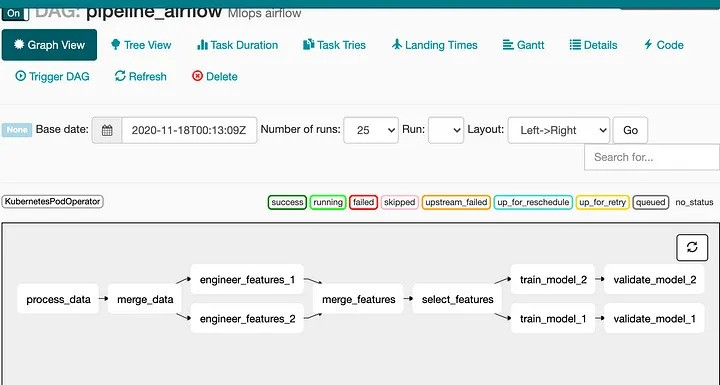
\includegraphics[scale=0.6]{Aairflow-pipeline.jpg}
	\caption{خط لوله در \lr{Apache Airlfow}}
	\label{fig: airflow pipelines}
\end{figure}

\subsubsection{انبار ویژگی}
انباره ویژگی\footnote{\lr{Feature Store}} یک سیستم مدیریت داده است که به منظور ذخیره‌سازی، مدیریت و اشتراک‌گذاری ویژگی‌های مورد استفاده در مدل‌های یادگیری ماشین طراحی شده است. این سیستم (شکل 
~\ref{fig: feature store})
دارای دو بخش اصلی است: پایگاه داده آنلاین و پایگاه داده آفلاین. هر یک از این پایگاه‌های داده نقش خاصی در فرآیند مدیریت و استفاده از ویژگی‌ها ایفا می‌کنند.

\textbf{پایگاه داده آفلاین}
برای ذخیره ‌سازی و مدیریت ویژگی‌هایی استفاده می‌شود که در فرآیندهای آزمایش و تحلیل به کار می‌روند. این پایگاه داده معمولاً با تاخیر نسبتا بیشتری نسبت به پایگاه داده آنلاین استفاده می شود و برای مواردی مناسب است که نیاز به پردازش حجم زیادی از داده‌ها در مدت زمان طولانی ‌تر دارند. ویژگی ‌هایی که در این پایگاه داده ذخیره می‌شوند، اغلب در فرآیندهای آموزش مدل‌های یادگیری ماشین مورد استفاده قرار می‌گیرند.

\textbf{پایگاه داده آنلاین}
برای ارائه ویژگی‌ها به صورت بلادرنگ استفاده می‌شود و تأخیر کمی دارد. این پایگاه داده‌ها برای سیستم‌هایی مناسب هستند که نیاز به پاسخگویی سریع دارند. زمانی که یک مدل یادگیری ماشین نیاز به استفاده از ویژگی‌ها برای انجام پیش‌بینی‌های فوری دارد، داده‌ها از این پایگاه داده آنلاین بازیابی می‌شوند. این نوع پایگاه داده‌ها باید توانایی پشتیبانی از حجم بالای درخواست‌ها را داشته باشند تا بتوانند عملکرد مطلوبی را در شرایط عملیاتی فراهم کنند. ویژگی‌هایی که در این پایگاه داده ذخیره می‌شوند، اغلب در فرآیندهای استنتاج مدل‌های یادگیری ماشین مورد استفاده قرار می‌گیرند.


با استفاده از انباره ویژگی توسعه‌دهندگان می‌توانند ویژگی‌های از پیش پردازش شده را به صورت متمرکز ذخیره کرده و به راحتی در پروژه‌های مختلف به اشتراک بگذارند، که این امر به تسریع فرآیند توسعه مدل‌ها و بهبود دقت پیش بینی ها کمک می‌کند. این سیستم‌ها معمولاً بر روی زیرساخت‌های ابری اجرا می‌شوند تا مقیاس‌پذیری بالا و کارایی مورد نیاز برای پردازش داده های کلان را فراهم کنند \cite{MLOpsCT2}. از ابزار معروف متن باز برای می توان به \lr{Feast}\cite{Feast} اشاره نمود.

\begin{figure}[t]
	\centering
	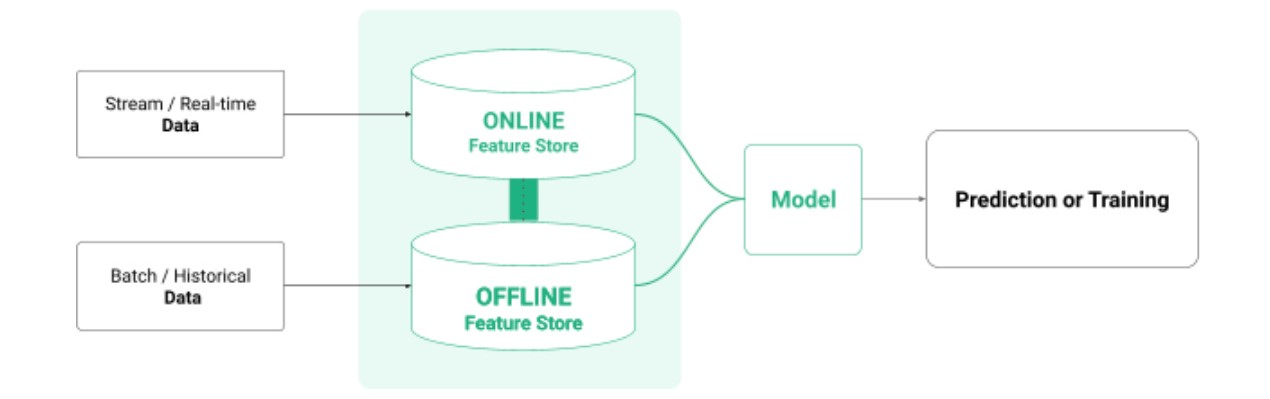
\includegraphics[scale=0.3]{feature-store2.jpg}
	\caption{انباره ویژگی}
	\label{fig: feature store}
\end{figure}

\subsubsection{بانک مدل}
بانک مدل\footnote{\lr{Model Registry}} یکی از ابزارهای بسیار مهم در مدیریت مدل‌های یادگیری ماشین است که به تیم‌ها کمک می‌کنند تا مدل‌های خود را به صورت سازماندهی شده ذخیره، مدیریت و ردیابی کنند. هم چنین اطلاعات مربوط به هر مدل را از جمله نسخه، تاریخ آخرین آموزش، معیارهای ارزیابی و مستندات مربوطه را نگهداری می‌کند. این امر به تیم‌ها کمک می‌کند تا با استفاده از نسخه‌های مختلف مدل‌ها، آزمایش‌های مختلفی انجام دهند و بهترین مدل را انتخاب کنند. هم چنین به هنگام بروز مشکل در مدل های جدید، می توان از مدل های قابل قبول قبلی برای محیط عملیاتی استفاده کرد \cite{MLOpsCloud1}. از ابزار معروف متن باز می توان به \lr{MLflow}\cite{MLflow} اشاره کرد.

\subsubsection{انبار فراداده}
انبار فراداده یادگیری ماشین\footnote{\lr{ML Metadata Store}} برای پیگیری و ذخیره‌سازی اطلاعات مربوط به هر مرحله از جریان کاری یادگیری ماشین استفاده می شوند. فراداده‌ها می‌توانند شامل جزئیاتی نظیر تاریخ و زمان آموزش مدل، مدت زمان هر مرحله از آموزش، پارامترهای استفاده شده، معیارهای عملکرد مدل، و سلسله‌مراتب مدل (مثل داده‌ها و کدهای استفاده شده) باشند. یکی از کاربردهای اصلی انبار فراداده‌ها، مدیریت کارآمد پروژه‌های پیچیده یادگیری ماشین است \cite{MLOpsProd2}. به عنوان مثال، در پروژه‌های بزرگ که شامل آزمایش‌ها و مدل‌های متعددی هستند، پیگیری دقیق و منظم فراداده‌ها می‌تواند به تیم‌ها کمک کند تا نتایج قبلی را به راحتی بازبینی کنند، مشکلات را شناسایی کنند و بهینه‌سازی‌های لازم را انجام دهند. \lr{MLflow}  یک ابزار معروف برای یک سیستم پیشرفته مدیریت فراداده است که همراه با بانک مدل امکان مدیریت یکپارچه مدل‌ها و فراداده‌ها را فراهم می‌کند. 	

\subsubsection{استقرار مدل}
استقرارکردن مدل\footnote{\lr{Model Serving}} به فرآیندی اشاره دارد که در آن مدل‌های یادگیری ماشین آماده برای استفاده، به کار گرفته می‌شوند تا به صورت عملیاتی به پیش‌بینی‌ها و استنتاج‌ها بپردازند. این فرآیند برای تبدیل مدل‌های آموزشی به ابزارهای قابل استفاده در محیط‌های تولیدی ضروری است و می‌تواند به صورت آنلاین برای پیش‌بینی‌های بلادرنگ یا به صورت دسته‌ای\footnote{\lr{Batch}} برای پردازش حجم بالای داده‌ها پیاده‌سازی شود. در محیط‌های عملیاتی، فرآیند استقرار مدل به سه شکل اصلی بلادرنگ، دسته ای و بدون سرور پیاده‌سازی می‌شود \cite{MLOpsCloud1}.

در استنتاج بلادرنگ\footnote{\lr{Real-time Inference}}، مدل‌های یادگیری ماشین به گونه‌ای پیاده‌سازی می‌شوند که بتوانند به سرعت و با کمترین تأخیر ممکن پیش‌بینی‌ها را انجام دهند. این نوع استنتاج برای کاربردهایی نظیر سیستم‌های توصیه‌گر، تحلیل داده‌های حسگرها و برنامه‌های کاربردی که نیاز به پاسخ‌های سریع دارند، مناسب است. به عنوان مثال، در سیستم‌های پیشنهاددهی محتوا مانند نتفلیکس یا آمازون، مدل‌ها باید به صورت بلادرنگ تحلیل کنند و پیشنهادهای شخصی‌سازی شده را ارائه دهند. تکنولوژی‌های مانند \lr{RESTful APIs} و \lr{gRPC} معمولاً برای پیاده‌سازی این نوع سرویس‌دهی استفاده می‌شوند.

استنتاج دسته‌ای\footnote{\lr{Batch Inference}} برای پردازش حجم وسیعی از داده‌ها به کار می‌رود که معمولاً به صورت زمان‌بندی شده انجام می‌شود. این روش برای تحلیل داده‌های کلان و پردازش‌های بزرگ مناسب است. به عنوان مثال، در تجزیه و تحلیل رفتار مشتریان یک فروشگاه آنلاین، داده‌های خریدهای گذشته می‌تواند به صورت دسته‌ای پردازش شود تا الگوهای مختلف شناسایی شود. ابزارهایی مانند \lr{Apache Spark}\cite{Spark} و \lr{Hadoop MapReduce}\lr{Hadoop} معمولاً برای پیاده‌سازی استنتاج دسته‌ای استفاده می‌شوند.

در استنتاج بدون سرور\footnote{\lr{Serverless Inference}}، مدل‌ها به صورت پویا و بر اساس تقاضا اجرا می‌شوند که هزینه و مقیاس‌پذیری را بهینه می‌کند. این نوع استنتاج زمانی مورد استفاده قرار می‌گیرد که نیاز به سرویس‌دهی مقیاس‌پذیر و مقرون‌به‌صرفه باشد. در استنتاج بدون سرور، مدل‌ها فقط زمانی که لازم است اجرا می‌شوند و بنابراین منابع بهینه‌سازی می‌شوند. سرویس‌های ابری مانند \lr{AWS Lambda} و \lr{Google Cloud Functions} معمولاً برای پیاده‌سازی این نوع استنتاج استفاده می‌شوند. از ابزارهای معروف متن باز برای استقرار مدل می توان به \lr{Knative}\cite{Knative} اشاره کرد. 

\subsubsection{نظارت}
نظارت\footnote{\lr{Monitoring}} در یادگیری ماشین یکی از مولفه‌های حیاتی برای تضمین عملکرد بهینه مدل‌ها و زیرساخت‌های مرتبط است. نظارت مداوم بر مدل‌های یادگیری ماشین به دلایلی از  جمله اطمینان از دقت پیش‌بینی‌ها، شناسایی ناهنجاری‌ها و بهبود مداوم عملکرد مدل‌ها ضروری است \cite{MLOpsData}. ابزارهایی مانند \lr{TensorBoard}،\lr{Kubeflow} و \lr{MLflow} نیز نقش مهمی در نظارت بر مدل‌های یادگیری ماشین ایفا می‌کنند. \lr{TensorBoard} به ویژه برای مصورسازی و تحلیل مراحل مختلف آموزش مدل‌ها مفید است. 

نظارت در یادگیری ماشین تنها به مدل‌ها محدود نمی‌شود؛ بلکه زیرساخت‌های مرتبط با یادگیری ماشین نیز نیاز به نظارت دارند. این نظارت شامل نظارت بر فرآیندهای \lr{CI/CD}، هماهنگی سرویس‌ها، خوشه های عملیاتی کوبرنتیز و گره های محاسباتی می‌شود \cite{MLOpsProd2}. یکی از ابزارهای رایج برای نظارت، \lr{Prometheus} است که به همراه \lr{Grafana} برای مصورسازی داده‌ها استفاده می‌شود. علاوه بر این پشته \lr{ELK} (\lr{Elasticsearch}, \lr{Logstash}, \lr{Kibana}) نیز یک مجموعه قدرتمند برای جستجو، تحلیل و مصورسازی لاگ‌های سیستم است که می‌تواند به شناسایی و رفع سریع مشکلات کمک کند. ابزارهای نظارتی به مهندسان اجازه می‌دهند تا هر گونه ناهنجاری در زیرساخت‌ها را به سرعت شناسایی و رفع کنند، که این امر موجب کاهش زمان از کار افتادگی سیستم و افزایش بهره‌وری می‌شود.
 
\subsubsection{زیرساخت آموزش و استقرار مدل}
این زیرساخت شامل منابع محاسباتی اصلی مانند واحد پردازش مرکزی، حافظه واحد پردازش گرافیکی\footnote{\lr{GPU}} است که برای پردازش داده‌ها و اجرای الگوریتم‌های پیچیده می باشد. زیرساخت ها می‌توانند به دو شکل توزیع شده\footnote{\lr{Distributed}} و غیرتوزیع شده پیاده‌سازی شوند. زیرساخت‌های غیرتوزیع‌شده معمولاً شامل ماشین‌های محلی هستند که با وجود سادگی در پیاده‌سازی، محدودیت‌هایی در مقیاس‌پذیری دارند. از سوی دیگر، زیرساخت‌های توزیع‌شده که معمولاً در بستر محاسبات ابری اجرا می‌شوند، امکان توزیع بار کاری بین چندین گره محاسباتی را فراهم می‌کنند و از این طریق مقیاس‌پذیری و کارایی بالاتری ارائه می‌دهند. یکی از ابزار محبوب برای مدیریت و سازآرایی محاسبات توزیع‌شده، کوبرنتیز است که امکان مدیریت کانتینرها و توزیع بار کاری بین گره‌ها را فراهم می‌کند. هم چنین، \lr{Red Hat OpenShift} نیز به عنوان یک پلتفرم دیگر شناخته می‌شود که قابلیت‌های مشابهی ارائه می‌دهد \cite{MLOpsCloud1}.

برای بهینه‌سازی عملکرد مدل‌های یادگیری عمیق، استفاده از واحد پردازش گرافیکی که برای ضرب ماتریسی بهینه‌سازی شده‌اند، استفاده می‌شوند. در دستگاه‌های لبه‌\footnote{\lr{Edge Devices}} به دلیل محدودیت‌های فضا، توان محاسباتی و مصرف انرژی، اجرای مدل‌های یادگیری عمیق پیچیده به چالش‌های خاصی مواجه است. برای غلبه بر این محدودیت‌ها و بهینه‌سازی عملکرد مدل‌ها در این دستگاه‌ها، تکنیک‌های مختلفی مورد استفاده قرار می‌گیرد. یکی از این تکنیک‌ها، استفاده از شبکه‌های عصبی کوانتیزه شده است. در کوانتیزاسیون، وزن‌ها و محاسبات شبکه عصبی از دقت کامل (به عنوان مثال، اعداد با دقت 32 بیت) به اعداد با دقت پایین‌تر (مانند 8 بیت یا حتی کمتر) کاهش می‌یابند. این کاهش دقت باعث کاهش حجم مدل و کاهش نیاز به منابع محاسباتی می‌شود. علاوه بر این، با استفاده از عملیات نقطه شناور کم‌دقت، می‌توان محاسبات را سریع‌تر و با مصرف انرژی کمتری انجام داد. تکنیک دیگر، هرس کردن\footnote{\lr{Pruning}} است که شامل حذف اتصالات غیرضروری و وزن‌های کوچک در شبکه عصبی می‌شود. این فرآیند باعث کاهش تعداد پارامترهای مدل می‌شود، بدون آنکه تاثیر قابل توجهی بر دقت مدل بگذارد. هرس کردن مدل را سبک‌تر و اجرای آن را سریع‌تر می‌کند، که این امر برای دستگاه‌های لبه‌ با منابع محدود بسیار مفید است.


\subsubsection{مخزن کد منبع}
مخزن کد منبع به عنوان یک نقطه مشترک برای نگهداری و مدیریت کدهای مربوط به مدل‌های یادگیری ماشین یک سازمان عمل می‌کند. با استفاده از سیستم‌های مدیریت نسخه مانند گیت، تیم‌ها می‌توانند به راحتی تغییرات کد را پیگیری کرده و در صورت لزوم به نسخه‌های قبلی کد بازگردند. این مخزن همچنین به خودکارسازی فرآیند \lr{CI/CD} کمک می‌کند، به طوری که هرگونه تغییر در کد به طور خودکار خط لوله را فعال کرده و  تغییرات تست، ارزیابی و در محیط‌های مختلف مستقر می‌شوند. می توان از ابزار متن باز برای پیاده سازی آن به \lr{GitLab}\cite{GitLab} و \lr{Gerrit}\cite{Gerrit} اشاره نمود.
\subsubsection{خط لوله \lr{CI/CD}}
همان طور که در گذشته نیز راجع به آن صحبت کردیم، خط لوله \lr{CI/CD} به تیم‌ها اجازه می‌دهند تا کدهای مدل و داده‌ها را به‌صورت مداوم تست، تأیید و استقرار دهند. در این فرآیند، مدل‌ها به طور خودکار بازآموزی و بهبود می‌یابند و در محیط‌های مختلف (توسعه، تست، تولید) به صورت پیوسته به‌روزرسانی می‌شوند. این کار نه تنها باعث افزایش کیفیت و دقت مدل‌ها می‌شود بلکه زمان توسعه و عرضه را نیز به طرز قابل‌توجهی کاهش می‌دهد. در \lr{MLOps} این خط لوله ‌ها در مراحل مختلف از جمله آموزش مدل، ارزیابی، استقرار و نظارت بر عملکرد مدل‌ها و هم چنین داده ها استفاده می‌شوند \cite{MLOpsProd2}. از ابزارهای مناسب برای این کار می توان به \lr{Jenkins}\cite{Jenkins} و \lr{GitLab CI}\cite{GitLab} نام برد. 

\subsection{نقش ها}
در تولید یک پلتفرم \lr{MLOps}، نقش‌های متعددی وجود دارد که همکاری آن‌ها برای طراحی، مدیریت، اتوماسیون و بهره‌برداری از سیستم‌های یادگیری ماشین در محیط تولید بسیار حیاتی است. در ابتدا سهام‌دار کسب‌وکار\footnote{\lr{Business Stakeholder}} وظیفه تعیین اهداف کسب‌وکار و استراتژی بازگشت سرمایه محصول یادگیری ماشین را بر عهده دارد. معمار، معماری سیستم را طراحی کرده و فناوری‌های مناسب را انتخاب می‌کند. دانشمند داده مسئله کسب‌وکار را به مسئله یادگیری ماشین ترجمه کرده و مدل‌ها را مهندسی می‌کند. مهندس داده خط لوله‌های داده و ویژگی را ایجاد و مدیریت می‌کند و داده‌ها را به درستی به سیستم‌های پایگاه داده و انبار ویژگی‌ها تزریق می‌کند. مهندس نرم‌افزار با استفاده از الگوهای طراحی، مسئله یادگیری ماشین را به یک محصول مهندسی‌شده تبدیل می‌کند. مهندس \lr{DevOps} خودکارسازی \lr{CI/CD}، سازآرایی جریان کاری یادگیری ماشین و استقرار مدل در تولید را تضمین می‌کند. در نهایت، مهندس \lr{MLOps} نقش ترکیبی از مهارت‌های چندگانه را دارد و زیرساخت یادگیری ماشین را ایجاد و مدیریت کرده، خط لوله‌های جریان کاری را خودکار می‌کند و مدل‌ها و زیرساخت را در تولید نظارت می‌کند.  این نقش ها که در شکل 
~\ref{fig: mlops roles}
نشان داده شده است، با همکاری و هماهنگی نزدیک می‌توانند \lr{MLOps} را به شکلی مؤثر و کارآمد پیاده‌سازی کنند، که نتیجه آن یک سیستم یادگیری ماشین پایدار و قابل اعتماد در محیط تولید خواهد بود. همکاری میان این نقش‌ها تضمین می‌کند که تمام جنبه‌های مربوط به توسعه، استقرار و نگهداری مدل‌های یادگیری ماشین به درستی مدیریت شود و به اهداف کسب‌وکار دست یابند.
\begin{figure}[t]
	\centering
	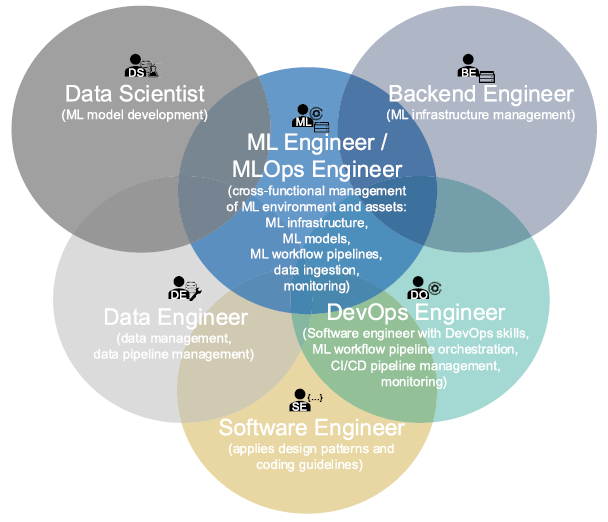
\includegraphics[scale=0.5]{mlops-roles.png}
	\caption{نقش ها و اشتراکات آنها در پارادایم \lr{MLOps}}
	\label{fig: mlops roles}
\end{figure}

\section{معماری جامع}
\begin{figure}[!b]
	\centering
	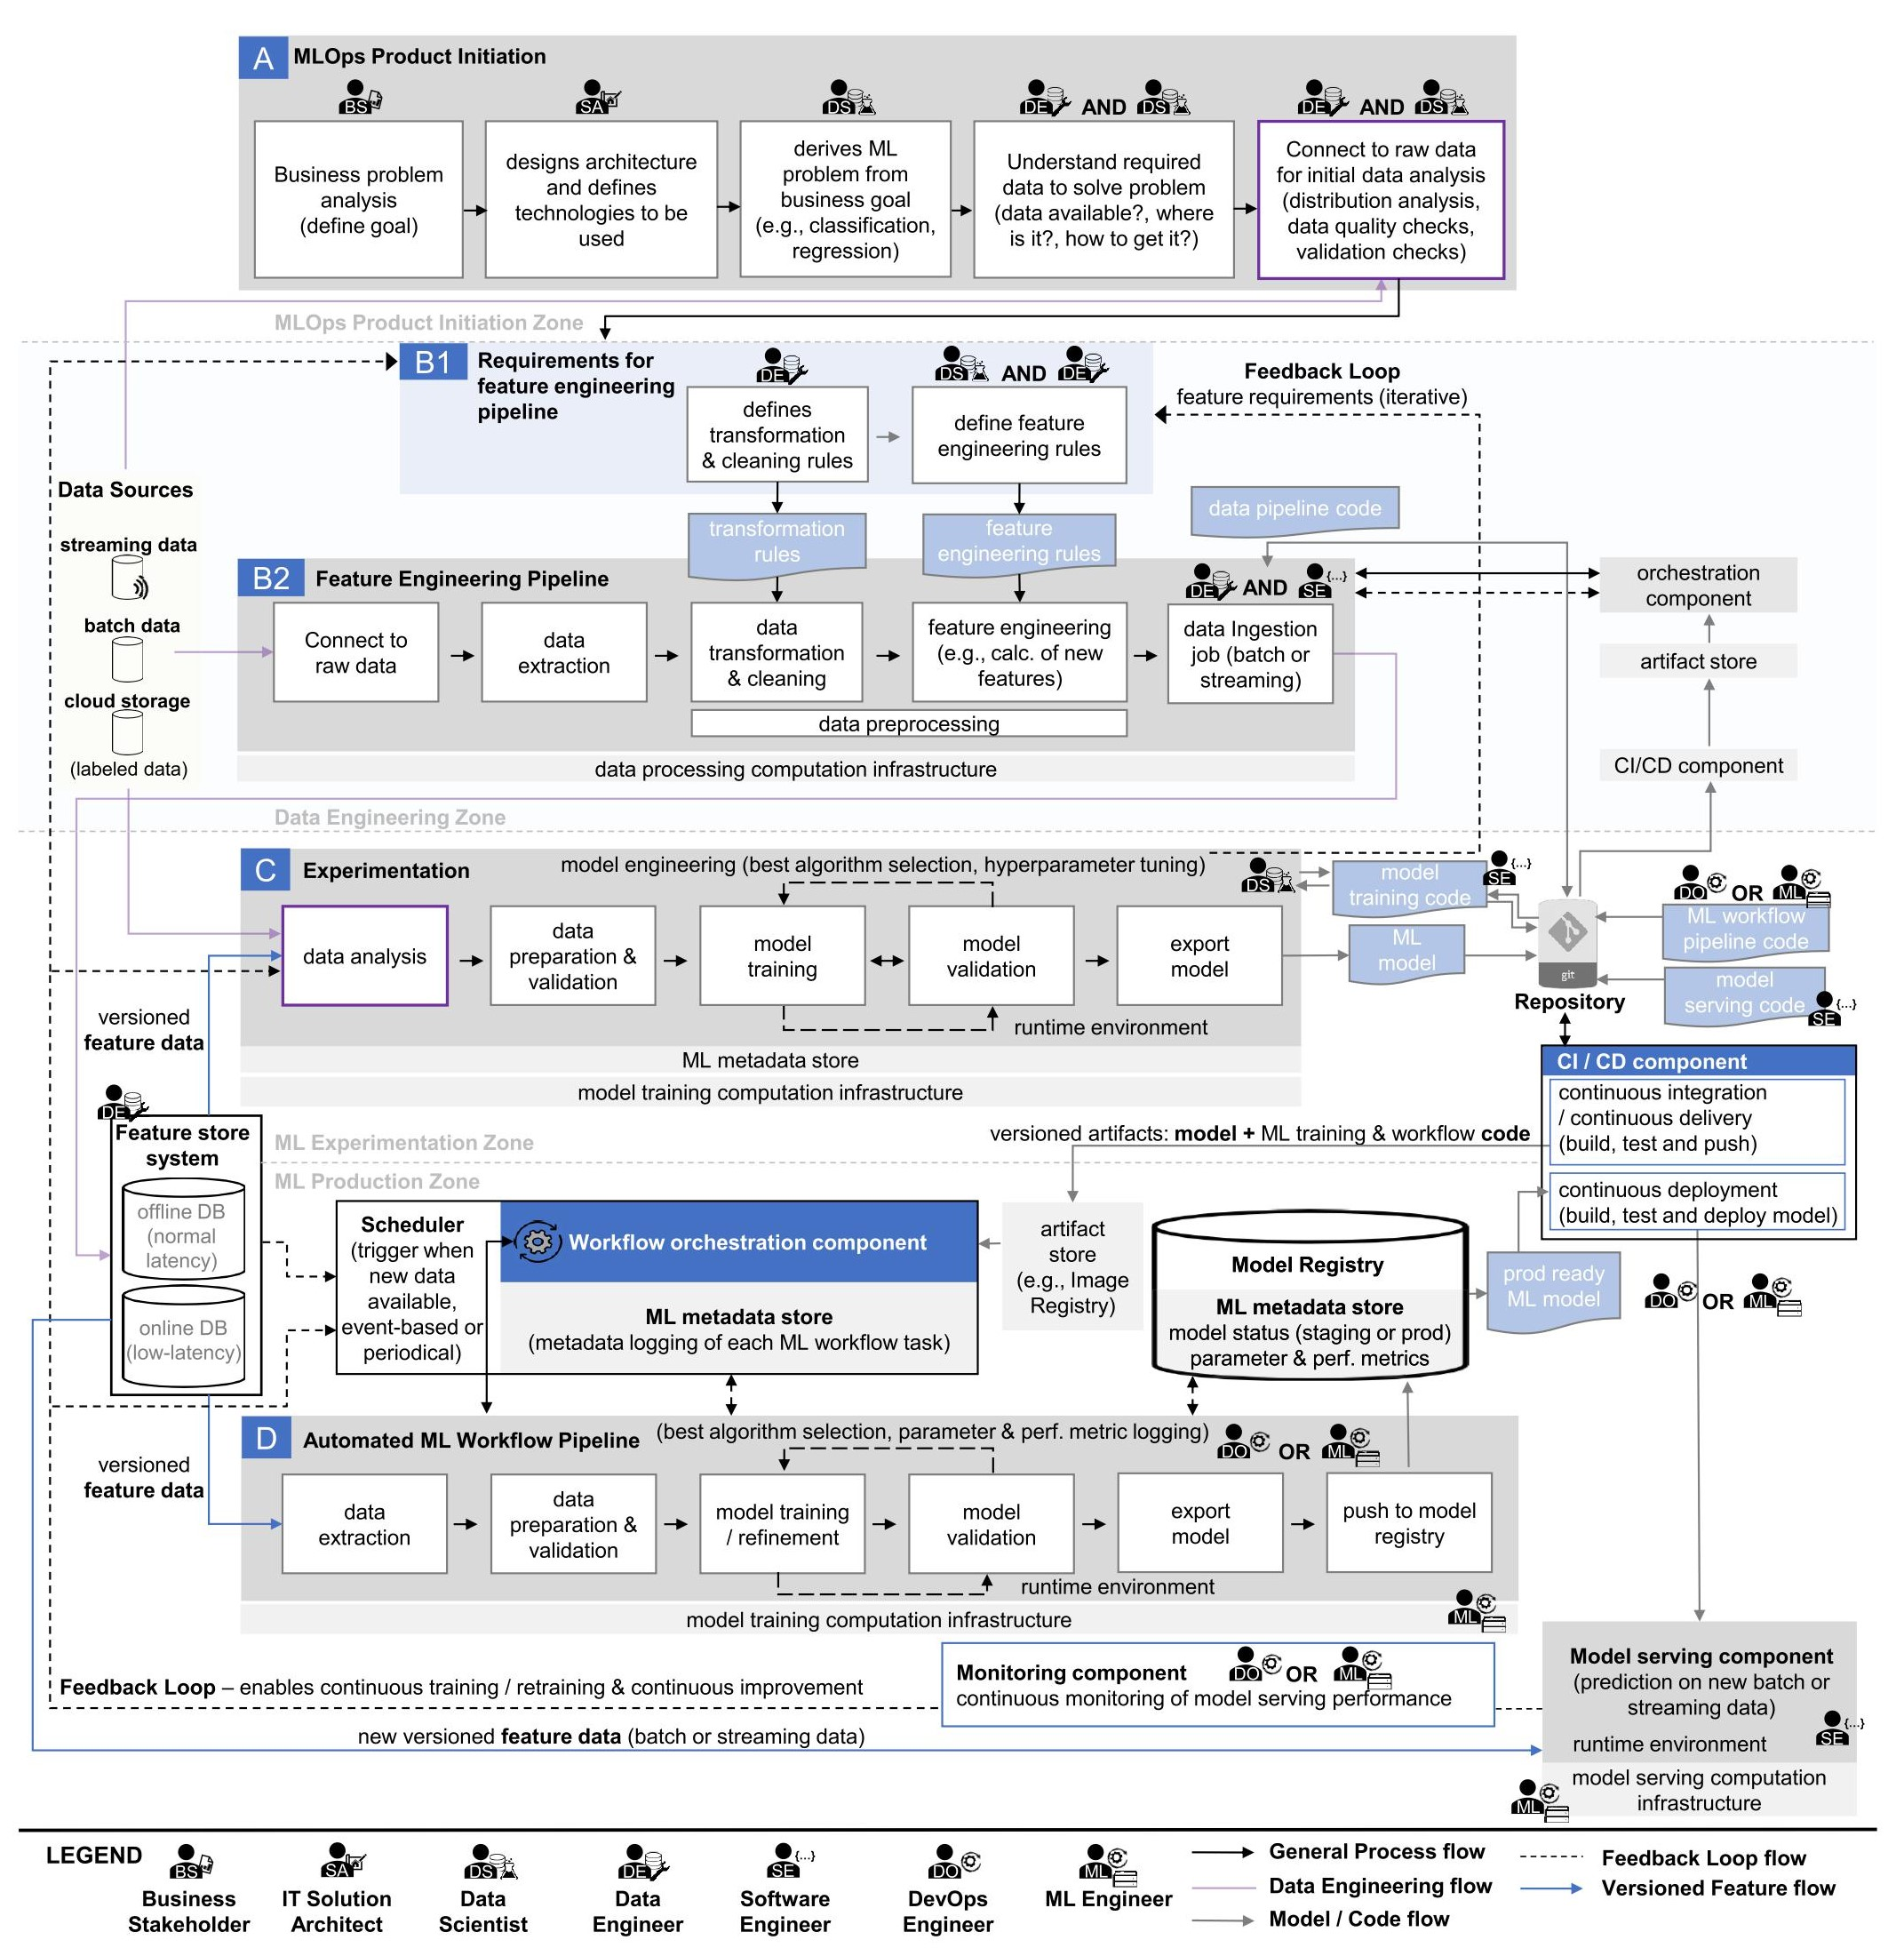
\includegraphics[scale=0.9]{mlops-architecture.jpg}
	\caption{معماری جامع \lr{MLOps}}
	\label{fig: mlops architecture}
\end{figure}
بر اساس اصول، اجزا و نقش‌های بیان شده، یک معماری جامع از یک پلتفرم \lr{MLOps} طراحی شده است. این معماری که در شکل 
~\ref{fig: mlops architecture}
 نشان داده شده جریان‌کارها و ترتیب وظایف در مراحل مختلف را ترسیم می‌کند. این معماری به‌گونه‌ای طراحی شده که کاربران می‌توانند مناسب‌ترین فناوری‌ها و چارچوب‌ها را بر اساس نیازهای خود انتخاب کنند. این انعطاف‌پذیری به کاربران این امکان را می‌دهد که پلتفرم \lr{MLOps} را با استفاده از ترکیبی از ابزارهای متن‌باز، استفاده از سرویس های ابری  یا رویکردهای ترکیبی پیاده‌سازی کنند. نرم‌افزارهای سازمانی و خدمات ابری اغلب از طریق \lr{API}‌ها با ابزارهای متن‌باز یکپارچه می‌شوند و امکان ترکیب بی‌دردسر فناوری‌های مختلف را فراهم می‌کنند. این معماری یک معماری جامع بوده و هر سازمان می تواند برحسب نیاز و هدف خود در حل مسئله یادگیری ماشین، این معماری را شخصی سازی کرده و از پیاده سازی قسمت هایی از آن صرف نظر کند.

\subsubsection{مرحله اولیه}
در فرآیند شروع محصول \lr{MLOps}، اولین مرحله با تحلیل کسب‌وکار آغاز می‌شود. کارشناس مریوط وظیفه دارد تا مشکلاتی را شناسایی کند که با استفاده از یادگیری ماشین قابل حل باشند. پس از شناسایی مشکل، معمار وارد عمل می‌شود. او طراحی معماری کلی سیستم یادگیری ماشین را تعریف کرده و پس از ارزیابی دقیق، تکنولوژی‌های مورد نیاز را انتخاب می‌کند. در مرحله بعدی، دانشمند داده وارد فرآیند می‌شود. دانشمند داده باید از هدف کسب‌وکار، یک مسئله یادگیری ماشین استخراج کند. این مسئله بسته به ماهیت مشکل کسب‌وکار می‌تواند شامل طبقه‌بندی، رگرسیون یا دیگر روش‌های یادگیری ماشین باشد. برای این منظور، دانشمند داده با همکاری مهندس داده باید داده‌های موجود را تجزیه و تحلیل کند تا بهترین رویکرد برای حل مسئله را انتخاب کند. این مرحله نیازمند دانش عمیق از روش‌های مختلف یادگیری ماشین و توانایی تطبیق آن‌ها با نیازهای خاص پروژه است. نکته مهم در این فرآیند، نیاز به داده‌های برچسب‌گذاری‌شده است که برای الگوریتم‌های نظارت‌شده ضروری هستند. در این معماری منابع داده از قبل دارای داده‌های برچسب‌گذاری‌شده بوده‌اند، زیرا فرآیند برچسب‌گذاری در مراحل قبلی انجام شده است.

\subsubsection{خط لوله مهندسی ویژگی}
در فرآیند توسعه مدل‌های یادگیری ماشین، مهندسی ویژگی‌ها\footnote{\lr{Feature Engineering}} به‌عنوان یکی از گام‌های حیاتی شناخته می‌شود که مستلزم تعیین نیازمندی‌های اساسی و پیاده سازی خط لوله مهندسی ویژگی‌ها است. این مرحله شامل تعریف و پیاده‌سازی قواعد تبدیل و پاک‌سازی داده‌ها، و همچنین ایجاد ویژگی‌های جدید و پیشرفته بر اساس ویژگی‌های موجود است. ابتدا نیازمندی‌های مهندسی ویژگی‌ها توسط متخصص داده و مهندس داده تعریف می‌شوند. در این مرحله، قواعد تبدیل داده‌ها\footnote{\lr{Data Transformation}} مانند نرمال‌سازی و تجمیع، و همچنین قواعد پاک‌سازی داده‌ها\footnote{\lr{Data Cleaning}} تعیین می‌شوند تا داده‌ها به فرمت قابل استفاده تبدیل شوند. این قواعد اولیه، به‌صورت تکراری و بر اساس بازخوردهای حاصل از مراحل آزمایشی مهندسی مدل و یا از طریق نظارت بر عملکرد مدل، تنظیم و بهبود می‌یابند.


با تعریف نیازمندی‌های اولیه، مهندس داده و مهندس نرم‌افزار اقدام به ساخت نمونه اولیه خط لوله تولید ویژگی‌ها می‌کنند. این خط لوله باید به صورت مداوم و بر اساس بازخوردهای دریافتی از مراحل مختلف، به‌روزرسانی و بهبود یابد. مراحل کلیدی پیاده‌سازی خط لوله تولید ویژگی‌ها به صورت زیر است:
\begin{itemize}
	\item 
اتصال به داده‌های خام:
اولین مرحله در پیاده‌سازی خط لوله تولید ویژگی‌ها، اتصال به منابع داده خام است. این داده‌ها می‌توانند از منابع مختلفی مانند داده‌های جریانی\footnote{\lr{Streaming Data}}، داده‌های دسته‌ای\footnote{\lr{batch data}} یا داده‌های ذخیره شده در ابر\footnote{\lr{Cloud Storage}}  باشند. داده‌های جریانی به صورت پیوسته و بلادرنگ دریافت می‌شوند، داده‌های دسته‌ای ثابت به صورت دوره‌ای و در حجم بالا جمع‌آوری و پردازش می‌شوند و داده‌های ذخیره شده در ابر از طریق سیستم‌های ابری مقیاس پذیر و انعطاف پذیر ذخیره می‌شوند. اتصال به منابع داده باید به گونه‌ای انجام شود که داده‌ها به راحتی قابل استخراج و پردازش باشند.
	\item 
استخراج داده‌ها:
پس از اتصال به منابع داده، مرحله بعدی استخراج داده‌ها از این منابع است. این مرحله شامل خواندن داده‌ها از پایگاه‌های داده، فایل های \lr{CSV} یا دیگر منابع داده است. 
	\item 
پیش ‌پردازش داده‌ها:
در این مرحله، داده‌های استخراج شده برای تبدیل به فرم قابل استفاده، پیش ‌پردازش می‌شوند. پیش‌ پردازش شامل مراحل مختلفی مانند پاکسازی داده‌ها، مدیریت مقادیر مفقود، حذف نویز، و نرمال‌سازی مقادیر است. هدف اصلی این مرحله، آماده‌سازی داده‌ها به گونه‌ای است که بتوانند به عنوان ورودی‌های مدل یادگیری ماشین استفاده شوند.
	\item 
استخراج ویژگی‌های جدید و پیشرفته: 
یکی از مهم‌ترین مراحل در خط لوله تولید ویژگی‌ها، استخراج ویژگی‌های جدید و پیشرفته است. این ویژگی‌ها بر اساس ویژگی‌های موجود و با استفاده از تکنیک‌های مختلفی مانند ترکیب ویژگی‌ها، اعمال توابع ریاضی، و بهره‌گیری از روش‌های آماری ایجاد می‌شوند. این مرحله به مدل یادگیری ماشین کمک می‌کند تا الگوهای پیچیده‌تری را در داده‌ها شناسایی کند و دقت پیش ‌بینی‌های خود را افزایش دهد.
	\item 
انتقال ویژگی ‌ها به انبار ویژگی‌ها:
در نهایت، داده‌های پردازش شده و ویژگی‌های محاسبه شده به انبار ویژگی‌ها وارد می‌شوند. این انبار می‌تواند شامل پایگاه‌های داده آنلاین یا آفلاین باشد. این بارگذاری باید به گونه‌ای انجام شود که دسترسی سریع و کارآمد به داده‌ها برای مراحل بعدی آموزش مدل فراهم شود.
\end{itemize}

در خط تولید ویژگی‌ها، مهندس نرم افزار به کمک مهندس داده کدهای مورد نیاز برای \lr{CI/CD} و سازآرایی را تعریف می‌کند تا وظایف خط تولید ویژگی‌ها به درستی هماهنگ شوند. این نقش شامل تنظیم منابع زیرساختی برای اطمینان از مقیاس پذیری و عملکرد بهینه خط تولید است. با این تنظیمات، خط تولید ویژگی‌ها می‌تواند به طور مداوم به‌روزرسانی شده و بر اساس بازخوردها بهبود یابد، که این امر بهبود عملکرد مدل‌های یادگیری ماشین را تضمین می‌کند.

برای پیاده‌سازی خطوط تولید ویژگی‌ها، از ابزارها و فناوری‌های مختلفی استفاده می‌شود. برخی از این ابزارها شامل \lr{Apache Spark}، \lr{Apache Kafka} و ابزارهای \lr{ETL} سنتی مانند \lr{Apache Airflow} هستند. \lr{Apache Spark} به دلیل توانایی بالای آن در پردازش موازی و تحلیل داده‌های بزرگ بسیار محبوب است. به عنوان مثال، در یک پروژه پردازش زبان طبیعی\footnote{\lr{Natural Language Processing}} با استفاده از اسپارک، داده‌های متنی بزرگ پردازش و ویژگی‌های متنی جدید محاسبه شدند \cite{MLOpsArchfeature1}. در پروژه دیگری در یک موسسه مالی، داده‌های اعتباری مشتریان با استفاده از اسپارک پردازش و ویژگی‌های مرتبط برای مدل ریسک اعتباری ایجاد شدند \cite{MLOpsArchfeature2}. 
\lr{Apache Kafka} \cite{Kafka} نیز برای بارگذاری داده‌های جریانی بلادرنگ به کار گرفته می‌شود.
هم چنین از \lr{Feast} به همراه پایگاه داده های معروف مانند \lr{PostgreSQL} و \lr{Redis} نیز برای انبار ویژگی ها استفاده می شود.
\subsubsection{بررسی و آزمایش}
مرحله آزمایش مدل در فرآیند یادگیری ماشین یک بخش حیاتی است که بیشتر توسط دانشمند داده به همراه مهندس نرم‌افزار انجام می‌شود. قبل از شروع به کار، مهندس داده به همراه مهندس نرم افزار برای اطمینان از عملکرد درست ابزار و منابع، محیط و سخت افزار را پیکربندی می کنند. حال فرآیند آزمایش مدل شروع می شود:
\begin{itemize}
	\item 
اتصال به انبار ویژگی: 
دانشمند داده به سیستم انبار ویژگی‌ ها متصل می‌شود تا داده‌ها را برای تجزیه و تحلیل دریافت کند. در صورت نیاز، داده خام نیز می‌تواند برای تحلیل‌های اولیه مورد استفاده قرار گیرد. اگر تغییراتی در داده‌ها لازم باشد، این تغییرات به تیم مهندسی داده گزارش می‌شود، که نتیجه آن می تواند منجر به تغییر قواعد تبدیل، پاک سازی داده ها و خط تولید ویژگی ها شود.
	\item 
آماده‌سازی و اعتبارسنجی داده‌ها: 
داده‌ها از سیستم انبار ویژگی‌ها جمع‌آوری و اعتبارسنجی می‌شوند. این مرحله شامل آماده‌سازی داده‌ها و تقسیم آنها به مجموعه‌های آموزش و تست و ارزیابی است تا مدل‌ها بتوانند به طور موثری آموزش داده شوند.
	\item 
آموزش و اعتبارسنجی مدل: 
در این مرحله، دانشمند داده الگوریتم‌های مختلف و پارامترهای آنها را ارزیابی می‌کند تا بهترین ترکیب را پیدا کند. آموزش مدل با استفاده از داده‌های آموزشی شروع می‌شود و مهندس نرم‌افزار در ایجاد کدهای آموزشی بهینه کمک می‌کند. مدل‌ها با استفاده از پارامترهای مختلف به صورت تعاملی آموزش و اعتبارسنجی می‌شوند. این فرآیند تکراری است و تا زمانی که مدل به عملکرد مطلوبی برسد، ادامه می‌یابد. هدف این مرحله شناسایی بهترین الگوریتم و پارامترهای بهینه است. 
	\item 
	استخراج مدل و ثبت کد: 
	پس از شناسایی و انتخاب بهترین مدل، دانشمند داده مدل نهایی را استخراج کرده و کدهای مربوطه را در مخزن کد منبع قرار می دهد. این کدها شامل تمامی اسکریپت‌ها و مستنداتی است که برای تولید، آموزش و ارزیابی مدل استفاده شده‌اند. در همین زمان، مهندس \lr{DevOps} یا مهندس یادگیری ماشین کدهای مربوط به خط لوله یادگیری ماشین را آماده و در مخزن قرار می دهد. این خط لوله شامل اسکریپت‌ها و تنظیماتی است که برای خودکارسازی فرآیندهای مختلف یادگیری ماشین مانند آموزش، ارزیابی و استقرار مدل مورد نیاز است. با انجام این کار، سیستم \lr{CI/CD} به صورت خودکار تغییرات را تشخیص داده و فرآیند ساخت، آزمون و تحویل مدل را آغاز می‌کند. در مرحله ساخت، مصنوعات مدل\footnote{\lr{Model Artifacts}} و کدهای مرتبط ایجاد می‌شوند. در مرحله آزمون، صحت و عملکرد مدل بررسی می‌شود و در نهایت، در مرحله تحویل مدل نهایی به مخزن مصنوعات ارسال می‌شود تا برای استفاده در محیط عملیاتی آماده باشد.	
\end{itemize}

در مرحله آزمایش، ابزارهای مبتنی بر \lr{Notebook} مانند \lr{Jupyter} \cite{Jupyter} به طور گسترده استفاده می‌شوند. این ابزارها به دانشمندان داده اجازه می‌دهند تا داده‌ها را آماده، مدل‌ها را آموزش، ارزیابی و بهینه‌سازی کنند. همچنین برای پیگیری و مدیریت آزمایش‌ها از ابزارهایی مانند \lr{MLflow} و \lr{TensorBoard} استفاده می‌شود.

\subsubsection{خودکارسازی جریان کاری یادگیری ماشین}
خودکارسازی جریان کاری یادگیری ماشین شامل مجموعه‌ای از فرآیندهای پیچیده و حیاتی است که توسط مهندس \lr{DevOps} و مهندس یادگیری ماشین مدیریت می‌شود. این فرآیندها شامل مدیریت محیط‌های اجرایی و زیرساخت‌های لازم برای آموزش مدل‌ها است که از منابع سخت‌افزاری و فریم‌ورک‌های محاسباتی نظیر کوبرنتیز استفاده می‌کنند. در این سیستم، یک مولفه ارکستراسیون وظایف مختلف را در جریان کاری خودکار یادگیری ماشین هماهنگ می‌کند. این مولفه وظایف را به محیط‌های مجزا (مانند کانتینرها) تخصیص داده و فراداده های هر وظیفه را در قالب لاگ‌ها، و سایر اطلاعات جمع‌آوری می‌کند. مراحل اجرای این فرآیند که به قسمت قبل خیلی شباهت دارد به صورت زیر است:
\begin{itemize}
	\item
استخراج داده‌ها:
	اولین مرحله در این فرآیند، استخراج داده‌ها از سیستم‌های انبار ویژگی‌ها است. این داده‌ها می‌توانند از پایگاه‌های داده آنلاین یا آفلاین استخراج شوند. بسته به نیاز مورد استفاده، داده‌ها از منابع مختلفی استخراج شده و برای مراحل بعدی آماده می‌شوند.
	\item
آماده‌سازی و اعتبارسنجی داده‌ها:
در این مرحله، داده‌ها به صورت خودکار آماده‌سازی و اعتبارسنجی می‌شوند. همچنین، تقسیم‌بندی داده‌ها به مجموعه‌های آموزش و تست نیز به صورت خودکار انجام می‌گیرد. این فرآیند تضمین می‌کند که داده‌های ورودی به مدل‌ها با کیفیت و قابل اعتماد باشند.
	\item
آموزش مدل نهایی:
پس از آماده‌سازی داده‌ها، مدل نهایی بر روی داده‌های جدید و نادیده آموزش داده می‌شود. الگوریتم‌ها و ابرپارامترها بر اساس تنظیمات مراحل آزمایشی قبلی از پیش تعریف شده‌اند. در این مرحله، مدل آموزش داده شده و بهینه‌سازی می‌شود تا بهترین عملکرد ممکن را ارائه دهد.
	\item
ارزیابی و تنظیم مدل:
	مدل آموزش‌دیده شده به صورت خودکار ارزیابی می‌شود و در صورت نیاز، ابرپارامترها تغییر می کنند. این فرآیند به صورت تکراری انجام می‌شود تا زمانی که معیارهای عملکرد نشان‌دهنده نتایج مطلوب باشند. این تکرارها تا دستیابی به یک مدل با عملکرد بهینه ادامه می‌یابند.
	\item
ثبت و ذخیره مدل:
	مدل نهایی آموزش‌دیده شده سپس ذخیره شده و به یک مخرن مدل منتقل می‌شود. این مخزن مدل، مدل‌ها را به صورت کد یا کانتینر همراه با فایل‌های تنظیمات و محیط ذخیره می‌کند. این امر تضمین می‌کند که مدل‌ها به راحتی قابل دسترسی و استفاده مجدد باشند.
\end{itemize}


برای هر بار آموزش مدل، مخزن فراداده ها پارامترهای مورد نیاز برای آموزش مدل و معیارهای عملکرد حاصل را ثبت می‌کند. این شامل ثبت جزئیات هر دوره آموزش مدل، مانند تاریخ و زمان آموزش، مدت زمان، پارامترهای استفاده شده و معیارهای عملکرد مدل می باشد. همچنین نسخه و وضعیت مدل (مثلاً آماده برای تولید یا در حال توسعه) نیز ثبت می‌شود.

پس از انتقال مدل با عملکرد بالا از مرحله آزمایش به تولید، این مدل به طور خودکار به مهندس \lr{DevOps} یا مهندس یادگیری ماشین برای استقرار مدل تحویل داده می‌شود. در این مرحله، ابزار مدیریت \lr{CI/CD} مانند \lr{ArgoCD}، خط لوله \lr{CD} را اجرا می‌کند. مدل آماده و کدهای استقرار مدل که توسط مهندس نرم‌افزار تهیه شده‌اند، فراخوانی می‌شوند. خط لوله \lr{CD} وظیفه ساخت و آزمایش مدل و کدهای استقرار مدل برای استقرار در محیط عملیاتی را بر عهده دارد. مؤلفه استقرار مدل مانند \lr{Knative} پیش بینی‌ها را بر اساس داده‌های جدید و دیده نشده از سیستم انبار ویژگی‌ها انجام می‌دهد. این مؤلفه می‌تواند توسط مهندس نرم‌افزار به صورت آنلاین برای پیش ‌بینی‌های زمان واقعی یا دسته‌ای برای داده های کلان طراحی شود. برای پیش بینی‌های زمان واقعی، ویژگی‌ها باید از پایگاه داده آنلاین با تأخیر کم دریافت شوند، در حالی که برای پیش بینی‌های دسته‌ای، ویژگی‌ها می‌توانند از پایگاه داده آفلاین با تأخیر معمولی دریافت شوند. برنامه‌های استقرار مدل اغلب با استفاده از یک کانتینر پیاده سازی و تنظیم می شوند و درخواست‌های پیش‌بینی را از طریق \lr{REST API} پاسخ می دهند. هنگام استقرار یک برنامه یادگیری ماشین، استفاده از آزمایش \lr{A/B} به عنوان یک استراتژی تست خوب توصیه می‌شود تا در یک سناریوی واقعی مشخص شود که کدام مدل بهتر عمل می‌کند.

مؤلفه نظارتی به صورت پیوسته عملکرد مدل و زیرساخت‌ها را پایش می کند. زمانی که یک آستانه خاص مانند کاهش دقت پیش بینی‌ها تشخیص داده شود، اطلاعات از طریق حلقه بازخورد ارسال می‌شود. این حلقه امکان آموزش و بازآموزی مداوم\footnote{\lr{Continuous Training (CT)}} و بهبود مستمر را فراهم می‌کند. اطلاعات از مؤلفه نظارتی مدل به چندین نقطه مانند مرحله آزمایش، مرحله تولید ویژگی و مهندسی داده منتقل می شود. بازخورد به مرحله آزمایش توسط دانشمند داده برای بهبود بیشتر مدل‌ها مورد استفاده قرار می‌گیرد. بازخورد به مرحله تولید ویژگی نیز امکان تغییر در تولید ویژگی‌های برای سیستم انبار ویژگی‌ها را فراهم می‌کند. تشخیص رانش داده به عنوان یک مکانیزم بازخورد نیز می‌تواند آموزش مستمر را فعال کند. رانش داده به تغییرات تدریجی یا ناگهانی در توزیع داده‌های ورودی مدل‌های یادگیری ماشین گفته می‌شود که می‌تواند باعث کاهش دقت و کارایی مدل‌ها شود. این تغییرات ممکن است به دلیل عوامل مختلفی مانند تغییر در رفتار کاربران، تغییر در شرایط محیطی، خرابی سنسورها و یا تغییرات سیستمی رخ دهند. رانش داده به دو نوع اصلی تقسیم می‌شود:

\textbf{رانش مفهوم}\footnote{\lr{Concept Drift}}:
 تغییر در توزیع برچسب‌ها یا خروجی‌ها که نشان دهنده تغییر در الگوهای زیرین داده‌هاست.
 
\textbf{رانش ویژگی}\footnote{\lr{Feature Drift}}
 تغییر در توزیع ویژگی‌ها یا ورودی‌های مدل که می‌تواند به دلیل تغییر در محیط یا منابع داده‌ها باشد.
 
تشخیص رانش داده اهمیت زیادی دارد زیرا به مدل‌ها کمک می‌کند تا با تغییرات جدید سازگار شوند و از کاهش کارایی جلوگیری کنند. این تشخیص می‌تواند از طریق مقایسه توزیع‌های آماری قدیم و جدید داده‌ها و استفاده از الگوریتم‌های مختلف انجام شود. هنگامی که رانش داده تشخیص داده شود، مدل‌ها می‌توانند مجدداً آموزش داده شوند تا با شرایط جدید سازگار شوند و کارایی مطلوب خود را حفظ کنند.

تکنولوژی‌ها و ابزار برای پیاده سازی خط لوله خودکار یادگیری ماشین شامل \lr{Apache Airflow} ، \lr{Kubeflow Pipelines} و \lr{AWS SageMaker} هستند. یک مثال از کاربرد صنعتی یک خط لوله خودکار یادگیری ماشین با استفاده از \lr{Airflow} در زمینه تبلیغات آنلاین است \cite{MLOpsArch3}. این شرکت از \lr{Airflow} برای خودکارسازی فرآیند آموزش و استقرار مدل‌های یادگیری ماشین برای هدف‌گذاری و بهینه‌سازی تبلیغات استفاده می کند. در این خط لوله، داده‌های بزرگی از منابع مختلف مانند داده‌های کلیک‌استریم وبسایت، جمعیت‌شناسی کاربران و داده‌های عملکرد کمپین استخراج، تبدیل و بارگذاری می‌شوند. این داده‌ها سپس از یک سری مراحل پیش‌پردازش و مهندسی ویژگی عبور می‌کنند که به‌عنوان اپراتورهای \lr{Airflow} پیاده‌سازی شده‌اند. در مرحله بعد، مدل‌های مختلف یادگیری ماشین بر روی داده‌های پردازش شده آموزش داده و ارزیابی می‌شوند. در نهایت، مدل با بهترین عملکرد برای تصمیم‌گیری‌های هدف‌گذاری تبلیغات بی‌درنگ به محیط تولید منتقل می‌شود. در این مثال، برای خودکارسازی کل فرآیند از جمله زمان‌بندی، نظارت و اجرای مجدد وظایف شکست‌خورده از \lr{Airflow} استفاده می‌شود.
\chapter{طراحی یگ پلتفرم \lr{MLOps}}
 
\section{مقدمه}
در این بخش می خواهیم مقدمه ای از طراحی و هدف آن بنویسیم

\section{سیستم مدیریت}
\subsection{خط لوله \lr{CI/CD}}

در دنیای فناوری اطلاعات، زیرساخت‌های تغییرناپذیر\footnote{\lr{Immutable Infrastructure}} و تغییرپذیر\footnote{\lr{Mutable Infrastructure}} دو رویکرد مهم در مدیریت و نگهداری سیستم‌ها هستند. زیرساخت‌های تغییرناپذیر به سیستم‌هایی اشاره دارند که پس از ایجاد، بدون تغییر باقی می‌مانند و در صورت نیاز به تغییر، سیستم های جدید جایگزین آنها می‌شوند. این رویکرد با مزایایی همچون کاهش پیچیدگی‌های مدیریتی، افزایش قابلیت پیش‌بینی و کاهش ریسک‌های مرتبط با تغییرات ناخواسته همراه است \cite{DevopsIaac2}. به کمک ابزارهایی مانند داکر و کوبرنتیز، پیاده‌سازی زیرساخت‌های تغییرناپذیر امکان‌پذیر است و از قابلیت مقیاس‌پذیری بالایی برخوردارند. سیستم‌های ابری غالباً از روش تغییرناپذیر استفاده کرده تا از مزایای آن بهره‌مند شوند. در مقابل، زیرساخت‌های تغییرپذیر به سیستم‌هایی اشاره دارند که می‌توانند به طور پویا تغییر کنند و تنظیمات و پیکربندی‌های جدید را بپذیرند. این رویکرد، انعطاف‌پذیری بیشتری را فراهم می‌کند و برای محیط‌هایی که نیاز به تغییرات مکرر دارند، مناسب‌تر است. با این حال، مدیریت تغییرات در زیرساخت‌های تغییرپذیر ممکن است چالش‌های بیشتری از جمله افزایش ریسک خطاها و نیاز به نظارت مداوم به همراه داشته باشد. انتخاب بین این دو رویکرد به نیازها و اولویت‌های سازمان بستگی دارد. در حالی که زیرساخت‌های تغییرناپذیر برای محیط‌های تولید با نیاز به ثبات و قابلیت پیش‌بینی بالا مناسب‌ترند، زیرساخت‌های تغییرپذیر برای محیط‌های توسعه و آزمایش که نیاز به انعطاف‌پذیری دارند، کاربرد بیشتری دارند \cite{DevopsIaac1}. 

با افزایش استفاده از سیستم‌های ابری و رویکرد تغییرناپذیر، مفهوم \lr{GitOps} معرفی شده است که از گیت برای مدیریت زیرساخت و پیکربندی بهره می‌برد. \lr{GitOps} توسط \lr{Weaveworks} در سال ۲۰۱۷ معرفی شد که رویکردی مدرن برای پیاده سازی خط لوله \lr{CD} بر روی سیستم های ابری است. در حالی که ابزارهای سنتی تحویل مداوم عمدتاً از مدل \lr{Push} استفاده می‌کنند، \lr{GitOps} مدل \lr{Pull} را معرفی می‌کند که به خصوص با کانتینرها و پیکربندی‌های اعلامی به خوبی کار می‌کند و آن را به یک روند محبوب در اکوسیستم بومی ابر تبدیل کرده است  \cite{Devopsgitops}. از معروف ترین ابزار کلیدی که فرآیندهای \lr{GitOps} را تسهیل می‌کند می توان به \lr{ArgoCD} اشاره کرد. 

\begin{figure}[t]
	\centering
	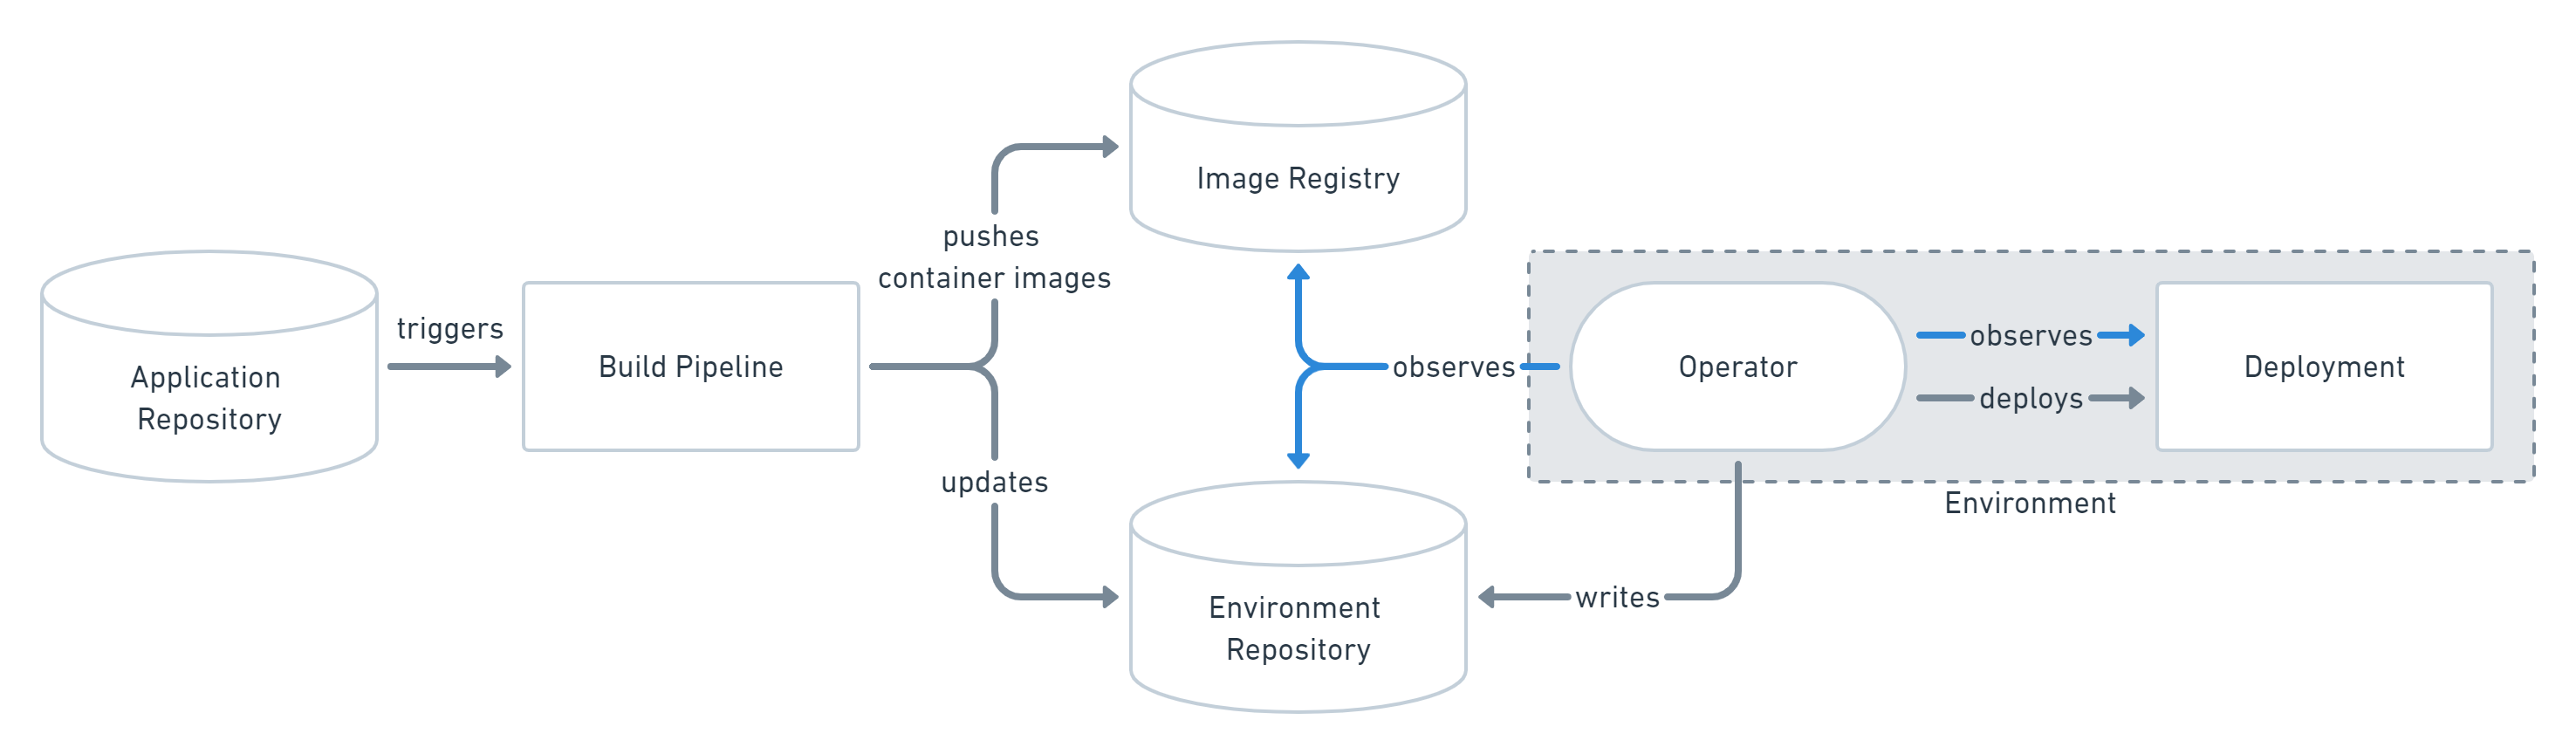
\includegraphics[scale=0.15]{gitops-pull.png}
	\caption{استقرار مبتنی بر \lr{Pull}}
	\label{fig: gitops pull}
\end{figure}

همان طور که گفته شد دو رویکرد در پیاده سازی خط لوله \lr{CD} وجود دارد. در مدل \lr{Pull} 
(شکل 
~\ref{fig: gitops pull})
مانند \lr{GitOps}، توسعه‌دهندگان حالت مطلوب را در مخزن گیت قرار می دهند. ابزاری نظیر \lr{ArgoCD} در محیط تولید به صورت خودکار این تغییرات را شناسایی کرده و اعمال می‌کنند. این مدل امنیت را افزایش می‌دهد زیرا نیازی به اعتبارنامه‌های دسترسی مستقیم برای توسعه‌دهندگان نیست. هم چنین این مدل مشکل استقرارهای مبتنی بر \lr{Push} را حل می کند، که در آن محیط تنها زمانی به روز می شود که مخزن محیط به روز شود. 
در مقابل، در مدل \lr{Push} (شکل 
~\ref{fig: gitops push})، استقرار در محیط تولید شامل خطوط لوله \lr{CI/CD} با اسکریپت‌هایی است که با هر تغییر در گیت فعال می‌شوند. این اسکریپت‌ها معمولاً ساخت، تست و در نهایت استقرار برنامه‌ها یا تنظیم پیکربندی‌های جدید در محیط تولید را با استفاده از ابزارهای خط فرمان و اعتبارنامه‌های ارائه شده انجام می‌دهند. این مدل کنترل دقیق‌تر بر فرآیند استقرار، اعمال سریع تغییرات، انعطاف‌پذیری بالا در مدیریت سناریوهای پیچیده و پشتیبانی بهتر از تغییرات جزئی را فراهم می‌کند، که در محیط‌های متنوع و پویا بسیار مفید است \cite{Devopsgitops}.
\begin{figure}[t]
	\centering
	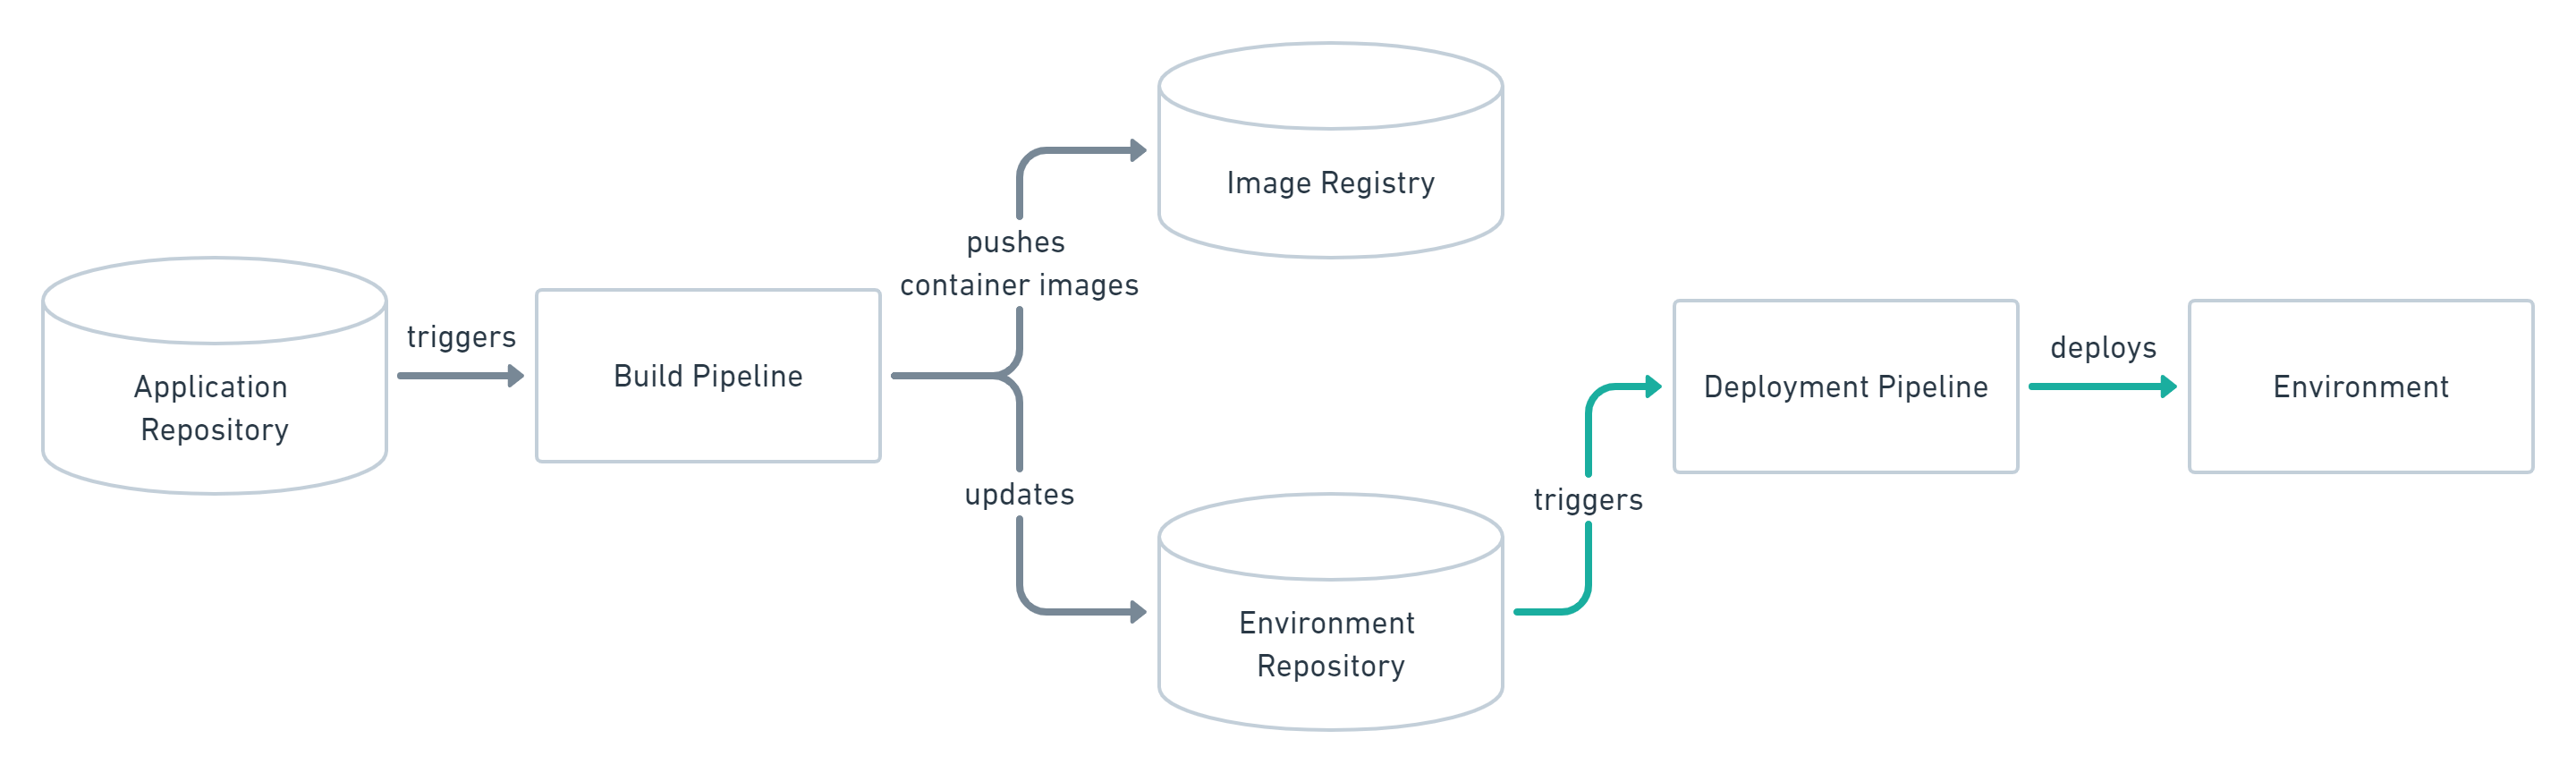
\includegraphics[scale=0.15]{gitops-push.png}
	\caption{استقرار مبتنی بر \lr{Push}}
	\label{fig: gitops push}
\end{figure}

به منظور پیاده‌سازی یک ابزار متن‌باز برای مدیریت خط لوله های \lr{CI/CD} که برای سیستم‌های ابری نیز مناسب باشد،  رویکرد تغییرپذیر  به همراه استراتژی استقرار مبتنی بر \lr{Push} انتخاب شده است. انتخاب رویکرد تغییرپذیر به دلیل نیاز به انعطاف‌پذیری بیشتر در محیط‌هایی که تغییرات مکرر و به‌روزرسانی‌های سریع دارند، انجام شده است. زیرساخت‌های تغییرپذیر به ما امکان می‌دهند تا به سرعت به تغییرات نیازمندی‌ها، پاسخ دهیم و تنظیمات و پیکربندی‌های جدید را به راحتی اعمال کنیم. این ویژگی در محیط‌های توسعه و آزمایش بسیار حیاتی است، زیرا تغییرات مداوم و آزمایش‌های متعدد بخشی از فرآیند توسعه نرم‌افزار هستند. هم چنین روش \lr{Push} نیز به دلیل سادگی و کارایی در اعمال به‌روزرسانی‌ها انتخاب شده است. با استفاده از این روش، می‌توانیم به‌روزرسانی‌ها را مستقیماً به سرورها ارسال کنیم و اطمینان حاصل کنیم که تمام سیستم‌ها به سرعت و بدون نیاز به مداخله دستی به‌روز می‌شوند. این رویکرد همچنین به کاهش زمان مورد نیاز برای انتشار تغییرات کمک می‌کند. در این راستا، \lr{Jenkins} به عنوان ابزار پیاده‌سازی و مدیریت خط لوله \lr{CI/CD} انتخاب شده است. جنکینز به دلیل متن‌باز بودن و دارا بودن تعداد زیادی پلاگین، انعطاف‌پذیری بسیار بالایی دارد و می‌تواند با انواع سیستم‌های ابری و رویکردهای زیرساختی سازگار شود. جنکینز همچنین با \lr{Ansible} که به عنوان ابزار مدیریت پیکربندی انتخاب شد، به خوبی سازگار است. این ترکیب به ما اجازه می‌دهد تا پیکربندی‌های پیچیده را به سادگی مدیریت کنیم و اطمینان حاصل کنیم که تمام زیرساخت‌ها به صورت هماهنگ عمل می‌کنند.
\subsubsection{طراحی خط لوله}
؟?????????
\subsection{مخزن کد منبع}

مخزن کد منبع\footnote{\lr{Source Code Repository}} یک سیستم ذخیره‌سازی و مدیریت کد است که به توسعه‌دهندگان این امکان را می‌دهد تا به صورت مشترک و هماهنگ بر روی پروژه‌های نرم‌افزاری کار کنند. این مخازن ابزارهای متعددی را برای تسهیل و بهبود فرآیند توسعه نرم‌افزار فراهم می‌کنند. یکی از اصلی‌ترین ویژگی های مخزن کد منبع، کنترل نسخه است که به توسعه‌دهندگان این امکان را می‌دهد تا تغییرات کد را پیگیری کرده و به نسخه‌های قبلی بازگردند. این ابزارها با ثبت تاریخچه تغییرات و شاخه‌بندی، امکان مدیریت همزمان چندین ویژگی یا رفع اشکال را فراهم می‌کنند بدون اینکه تغییرات یکدیگر را تحت تأثیر قرار دهند.

رایج‌ترین و پرکاربردترین این مخازن، گیت است که با ابزارهای مختلفی مانند \lr{GitHub}، \lr{GitLab} و \lr{Bitbucket} یکپارچه می‌شود. از آنجایی که یکی از شرط های پیاده سازی پلتفرم، متن باز بودن ابزار های آن می باشد، \lr{GitLab} برای مدیریت مخزن کد منبع استفاده شده است. در این طراحی \lr{Jenkins} به \lr{GitLab} به عنوان مخزن کد متصل شده و هر تغییر در کد منبع باعث اجرا شدن یک خط لوله \lr{CI/CD} مشخص توسط \lr{Jenkins} می گردد.

\subsection{مخزن مؤلفه ها}
یک مخزن مؤلفه\footnote{\lr{Artifact Repository}} یک سیستم متمرکز برای ذخیره‌سازی، مدیریت و انتشار مؤلفه های نرم‌افزاری است. این مؤلفه ها شامل هر نوع فایل باینری، کتابخانه، ماژول، پکیج، پلاگین یا حتی مستنداتی می‌شود که در طول چرخه عمر توسعه نرم‌افزار تولید می‌شود. هدف اصلی این مخازن این است که به تیم‌های توسعه اجازه دهد تا به راحتی نسخه‌های مختلفی از مؤلفه ها را مدیریت و به اشتراک بگذارند، فرآیندهای ساخت و انتشار را ساده کنند و وابستگی‌ها را طور موثرتری مدیریت کنند. همچنین، از انتشار مؤلفه هایی که هنوز تست نشده‌اند یا از نظر امنیتی مشکلاتی دارند جلوگیری می‌کنند. 
یکی از ابزارهای محبوب و متن باز برای مدیریت مخازن مؤلفه ها، \lr{Nexus} است. \lr{Nexus} از فرمت‌های مختلف مؤلفه ها مانند \lr{Helm}، \lr{apt}، \lr{PyPI} و \lr{Docker} پشتیبانی می‌کند، که این امر آن را به یک ابزار چندمنظوره برای انواع پروژه‌های نرم‌افزاری تبدیل می‌کند. مخازن مؤلفه موردنیاز برای پیاده سازی پلتفرم در 4 نوع \lr{raw}، \lr{apt}، \lr{PyPI} و \lr{Docker} می باشد.

\subsubsection{مخازن \lr{APT}}
یک سیستم مدیریت بسته در سیستم‌عامل‌های مبتنی بر دبیان است که به کاربران اجازه می‌دهد تا بسته‌های نرم‌افزاری را به راحتی نصب، به‌روزرسانی و حذف کنند. از آنجایی بسته های استفاده شده در سرور ها غالبا یکسان می باشد، به منظور افزایش سرعت پیاده سازی و اعمال تغییرات و پیکربندی تمامی بسته های مورد استفاده و نصب نشده در محیط، در \lr{Nexus} ذخیره خواهند شد. این امر با استفاده از مخازنی از نوع \lr{Proxy} انجام خواهد شد. در پیاده سازی سیستم علاوه بر بسته های موجود در \lr{APT} رسمی \lr{Ubuntu}، از مخازن \lr{Containerd} و \lr{Kubernetes} نیز برای نصب و پیاده سازی کوبرنتیز نیز استفاده شده است. علاوه بر این، یک مخزن هم برای نصب \lr{Nvidia Driver} و \lr{Nvidida CUDA Toolkit} برای استفاده از واحد پردازنده گرافیکی ایجاد خواهد شد.
\subsubsection{مخزن \lr{PyPI}}
	یک مخزن عمومی برای بسته‌های نرم‌افزاری پایتون است که به توسعه‌دهندگان اجازه می‌دهد تا کتابخانه‌ها و ابزارهای خود را منتشر، به‌روزرسانی و مدیریت کنند. کاربران می‌توانند این بسته‌ها را به‌راحتی با استفاده از ابزار \lr{pip} نصب کنند. همانند \lr{APT}، به منظور ذخیره سازی تمامی بسته های استفاده شده در محیط تولید ساخته شده اند. این امر باعث افزایش سرعت در نصب مجدد بسته ها و پایداری سیستم در زمان های قطعی یا خرابی مخازن رسمی می شود.
\subsubsection{مخزن \lr{Docker}}
	یک سرویس برای \lr{Docker Images} است که به توسعه‌دهندگان اجازه می‌دهد تا تصاویر خود را ذخیره، مدیریت و به اشتراک بگذارند. با توجه به تحریم استفاده از \lr{DockerHub} در ایران وهم چنین کند بودن راه های جایگزین در گرفتن تصاویر موردنظر از مخازن رسمی این مخزن به وجود آمده که به مخزن رسمی \lr{docker.io} پراکسی شده است. علاوه بر این تصاویر لازم برای پیاده سازی و پیکربندی محیط که با خط لوله \lr{CI/CD} ساخته شده اند نیز برای استفاده مجدد در این مخازن قرار می گیرند.
\subsubsection{مخزن \lr{raw}}
	برای ذخیره‌سازی و مدیریت فایل‌ها و داده‌هایی استفاده می‌شود که فرمت خاصی ندارند. این نوع مخزن به توسعه‌دهندگان اجازه می‌دهد تا انواع مختلف فایل‌ها، مانند اسکریپت‌ها، تصاویر، و مستندات را بدون نیاز به ساختاردهی خاصی نگهداری کنند.


شکل از نکسوس بگذار ؟؟؟؟؟؟؟؟؟؟؟؟؟؟؟؟؟؟؟؟؟؟؟؟؟؟؟؟؟؟؟؟؟؟؟؟؟؟؟؟؟؟؟؟؟؟؟؟؟؟؟











\chapter{نتیجه‌گیری و پیشنهادات} \label{ch:Conclusion}

ما یک پلتفرم \lr{MLOps} متن‌باز و مبتنی بر ابر طراحی کرده‌ایم که خودکارسازی و بازتولید را در اکثر مراحل فرآیند یادگیری ماشین فراهم می‌کند. این پلتفرم در محیط‌های کوبرنتیز ارائه‌دهندگان مختلف ابری، کوبرنتیز داخلی و کوبرنتیز شبیه‌سازی شده روی ماشین‌های محلی اجرا می‌شود. هدف این طراحی، ایجاد زیرساختی است که مناسب اکثر پروژه‌ها و تیم‌های یادگیری ماشین باشد و فرآیندهای آن‌ها را به صورت خودکار و مقیاس‌پذیر نماید. 

محدودیت‌های فعلی و کارهای آینده شامل چندین بهبود مهم است که باید در پلتفرم \lr{MLOps} ما اعمال شود. در حال حاضر، فرآیندهای بازآموزی توسط یک وب‌هوک ساده تحریک می‌شوند که نیازمند یک اپراتور سفارشی برای مدیریت هوشمندانه‌تر چرخه‌ها و جلوگیری از بازآموزی‌های مکرر است. همچنین، پلتفرم برای اجرا به زیرساختی با منابع سخت‌افزاری زیاد نیاز دارد که توسعه محلی را دشوار و هزینه‌های سخت‌افزاری را افزایش می‌دهد؛ بنابراین، بهینه‌سازی‌های بیشتری برای سبک‌تر کردن پلتفرم ضروری است. بهینه‌سازی سرویس مش با جایگزینی \lr{Istio} با یک سرویس مش سبک‌تر، ادغام استفاده از سرویس مش با سرویس های کوبرنتیز به منظور افزایش سرعت پاسخ دهی به درخواست کاربر و کاهش اجزای غیرضروری \lr{Knative-Serving} نیز مورد نیاز است. امنیت سایبری پلتفرم باید تقویت شود و یک مطالعه موردی برای ارزیابی عملکرد و قابلیت اجرایی پلتفرم با پیاده‌سازی سیستم‌های یادگیری ماشین پیچیده و پرمنبع مانند آموزش مدل‌های زبانی بزرگ انجام شود. بهبودهای آینده شامل توسعه مرحله مدیریت شده برای برچسب‌گذاری داده‌ها، بهبودهای رابط کاربری برای ساده‌سازی استفاده از پلتفرم و ایجاد فرم‌های رابط کاربری برای افزودن استقرارها، جریان‌های کاری و تحریک‌ها است.



% شروع مراجع %%%%%%%%%%%%%%%%%%%%%%%%%%%%%%%%%%%%%%%
% References
\begin{latin}
\renewcommand{\bibname}{\rl{مراجع}}
\bibliography{SepSrc}
% یکی از دو دستور زیر را فعال کنید. به نظر من برای یک تز یا یک کتاب باید مراجع به ترتیب الفبایی اسم نویسنده اول مرتب شوند، و مرتب کردن به ترتیب ارجاع در متن برای مقاله است.
\bibliographystyle{IEEEsort} % مرتب کردن مراجع به ترتیب حروف الفبای اسم نویسنده اول
%\bibliographystyle{IEEEbib}  % مرتب کردن مراجع به ترتیب ارجاع در متن
\end{latin}

% شروع قسمتهای انتهایی تز (چکیده انگلیسی و جلد انگلیسی) %%%%%%%%%%%%%%%%
\thispagestyle{empty}


\phantom{a}
\vfil

\begin{latin}
\centering
\begin{minipage}{0.9\textwidth}
{

%\noindent \rule{\textwidth}{2pt}

\noindent {\bf ABSTRACT}
\vskip 2mm

\baselineskip=0.4\baselineskip
In the digital world today, invisible and robust image watermarking which embeds invisible signals
in to the digital images has been proposed as a major solution to the problem of copyright protection 
of digital images. Several approaches such as exploiting Human Visual System (HVS) and invariant domain
watermarking have been proposed to achieve this goal. In this thesis we use the information-theoretic
concepts as tools to develop methods for embedding watermark in an optimized way. Also multi-resolution 
transforms such as wavelet transform and MR-SVD (Multi-Resolution form of the Singular Value Decomposition)
are used in the proposed structure, because theses transforms resemble the HVS characteristics  for an
optimized watermarking  structure. Entropy concept and entropy~masking effects were proposed to use to develop
a model in DWT domain to increase the strength and robustness of the watermark, while perceived quality
of the electronic image is not altered. 
Then, the structure similar to the entropy-based proposed structure in DWT domain, 
is used for watermarking in the MR-SVD transform domain, which is found a new approach to robust image 
watermarking. Simulation results show that the proposed methods outperform conventional methods
in terms of both invisibility and robustness.  \\
\baselineskip=2\baselineskip

\vspace{15mm}

\noindent {\bf KEYWORDS}
\vskip 2mm

{
1. Image Watermarking. \\
2. Multi-Resolution Transform.\\
3. Human Visual System (HVS).\\
4. Wavelet Transform.\\
5. Singular Value Decomposition (SVD).\\
6. Entropy.\\
7. Entropy Masking.\\
}
}
\end{minipage}
\end{latin}
\vfil
  

\thispagestyle{empty}

\begin{latin}
\centering
\vspace*{-2.5cm}

\includegraphics[width=4cm]{Sharif_Logo.pdf}
\vspace*{-1.5cm}

{\large \bf SHARIF UNIVERSITY OF TECHNOLOGY} \\
{\bf ELECTRICAL ENGINEERING DEPARTMENT}

\vspace{2cm}

{\large \bf M.Sc. THESIS}
\vskip 1cm
{\sl Title:}\\

\baselineskip=2\baselineskip
{\huge \bf 

An Information-Theoretic Model for Image Watermarking
}\par

%\vspace{1.5cm}  % 1.2cm If both HAMKAAR and MOSHAVER exist
\vfil

by:\\
\vspace{-2mm}
{\large \bf AAAAA   BBBBBB}

%\vspace{2cm} % 1.1cm If both HAMKAAR and MOSHAVER exist
\vfil

{\sl Supervisor:}\\
\vspace{-1mm}
{\large \bf Dr. \dots\\}

%\vfil
%{\sl Co-supervisor:}\\
%\vspace{-1mm}
%{\large \bf  Dr. \dots\\}

%\vfil

%{\sl Advisor:}\\
%\vspace{-1mm}
%{\large \bf  Dr. \dots\\}

\vfil

{August 2005}
\par
\end{latin}



%%%%%%%%%%%%%%%%%%%%%%%%%%%%%%%%%%%%%%%%%%%%%%%%%%%%
\end{document}
